\author{João Gonçalves}
\newcommand{\authorD}{Daniel Dinis}
\newcommand{\authorM}{Diogo Costa}
\newcommand{\studentID}{99995}
\newcommand{\studentIDD}{99906}
\newcommand{\studentIDM}{99919}
\newcommand{\supervisorone}{Prof\textsuperscript{\underline{a}}. Stefânia de Sousa Faria}
\newcommand{\supervisortwo}{}
\newcommand{\department}{Engenharia Eletrotécnica e de Computadores}
\newcommand{\exam}{Telecomunicações}

\title{%
\LARGE 2\textsuperscript{\underline{o}} Trabalho Laboratorial\\
\Large Análise de sistemas BPSK e QPSK:\\
\large Impacto do AWGN na taxa de erro de bit}
\date{Novembro 2022}

\documentclass[a4paper,12pt]{article}
\usepackage[left=30mm,top=30mm,right=30mm,bottom=30mm]{geometry}
\usepackage[bottom]{footmisc}
\usepackage{etoolbox}
\usepackage{pgfplots}
\usepackage{circuitikz}
\usepackage{booktabs}
\usepackage[usestackEOL]{stackengine}
\usepackage[T1]{fontenc}
\usepackage[utf8]{inputenc}
\usepackage{bm}
\usepackage[export]{adjustbox}
\usepackage{graphicx}
\usepackage[font=footnotesize]{caption}
%\usepackage{caption}
\usepackage{subcaption}
\usepackage{amsmath}
\usepackage{amsfonts}
\usepackage{mathtools}
\usepackage{float}
\usepackage[linktoc=all]{hyperref}
\usepackage[capitalise]{cleveref}
\usepackage{enumitem,kantlipsum}
\usepackage[square,numbers,sort]{natbib}
\usepackage[ruled,vlined]{algorithm2e}
\usepackage{listings}
\usepackage{minted}
\usepackage{amssymb}
\usepackage{babel}
\usepackage[nottoc,numbib]{tocbibind}
\usepackage{tcolorbox}
\usepackage{xcolor}
\usepackage{graphicx,array}
\usepackage{breakurl}
\usepackage{placeins}
\usepackage{colortbl}
\def\UrlBreaks{\do\/\do-}
%\tcbuselibrary{skins,breakable}
%\usetikzlibrary{shadings,shadows}
\settocbibname{Referências}
\usemintedstyle{emacs}
%\setlength{\parindent}{0pt}

\newenvironment{block}[1]{%
    \tcolorbox[beamer,%
    noparskip,breakable,
    colback=LightBlue,colframe=DarkBlue,%
    colbacklower=DarkBlue!75!LightBlue,%
    title=#1]}%
    {\endtcolorbox}

\renewcommand{\figurename}{Fig.}
\renewcommand{\tablename}{Tab.}
\renewcommand{\contentsname}{Índice}

\hypersetup{
    colorlinks,
    linkcolor={black},
    citecolor={blue!50!black},
    urlcolor={blue!80!black}
}

\linespread{1}

\newtheorem{theorem}{Theorem}[section]
\graphicspath{{figures/}}	

\newcolumntype{C}[1]{>{\centering\let\newline\\\arraybackslash\hspace{0pt}}m{#1}}
\newcolumntype{L}[1]{>{\raggedright\let\newline\\\arraybackslash\hspace{0pt}}m{#1}}

\def\delequal{\mathrel{\ensurestackMath{\stackon[1pt]{=}{\scriptstyle\Delta}}}}

\expandafter\def\expandafter\UrlBreaks\expandafter{\UrlBreaks\do\a%
\do\b\do\c\do\d\do\e\do\f\do\g\do\h\do\i\do\j\do\k\do\l\do\m\do\n%
\do\o\do\p\do\q\do\r\do\s\do\t\do\u\do\v\do\w\do\x\do\y\do\z\do\&}
%---
\DeclareCaptionFont{white}{\color{white}}
\DeclareCaptionFormat{listing}{\colorbox{black}{\parbox{\textwidth}{#3}}}
\captionsetup[lstlisting]{format=listing, labelfont=white, textfont=white}
\lstdefinestyle{1}{% setup listings
    language=python,% set programming language
    inputencoding=latin1,
    basicstyle=\fontsize{7pt}{7pt}\ttfamily,
    keywordstyle=\color{blue},% keyword style
    commentstyle=\color{gray},% comment style
    numbers=left,% display line numbers on the left side
    numberstyle=\fontsize{7pt}{0pt},% use small line numbers
    numbersep=10pt,% space between line numbers and code
    tabsize=2,% sizes of tabs
    showstringspaces=false,% do not replace spaces in strings by a certain character
    captionpos=t,% positioning of the caption above
    breaklines=true,% automatic line breaking
    escapeinside={(*}{*)},% escaping to LaTeX
    fancyvrb=true,% verbatim code is typset by listings
    extendedchars=true,% prohibit extended chars (chars of codes 128--255)
    literate={"}{{\texttt{"}}}1 {á}{{\'a}}1 {é}{{\'e}}1 {í}{{\'i}}1 {ó}{{\'o}}1 {ú}{{\'u}}1 {ç}{{\c{c}}}1 {ã}{{\~a}}1 {õ}{{\~o}}1 {à}{{\`a}}1 {À}{{\`A}}1 {Á}{{\'A}}1 {É}{{\'E}}1 {Í}{{\'I}}1 {Ó}{{\'O}}1 {Ú}{{\'A}}1 {~}{{$\bm\sim$}}1 {<=}{{$\bm\le$}}1{>=}{{$\bm\ge$}}1{!=}{{$\bm\neq$}}1 {^}{{$^{\bm\wedge}$}}1 ,% item to replace, text, length of chars
    alsoletter={.<-},% becomes a letter
    alsoother={$},% becomes other
    otherkeywords={!=, ~, $, \&, \%/\%, \%*\%, \%\%, <-, <<-, /},% other keywords
    deletekeywords={de, R}% remove keywords
}
\lstset{style=1}
%----------------------------------TITLE PAGE -----------------------------------
\makeatletter
\def\maketitle{
  \begin{center}\leavevmode
       \normalfont
       
\includegraphics[width=0.55\columnwidth]{IST.pdf}
       \vskip 1.5cm   
       \textsc{\large \department}\\
       \vskip 1.5cm
       \rule{\linewidth}{0.2 mm} %\\
       {\large \exam}\\[1 cm]
       {\huge \bfseries \@title \par}
       \vspace{1cm}
	\rule{\linewidth}{0.2 mm} \\[1.5 cm]
	 
	\begin{minipage}[t]{0.45\textwidth}
		\begin{flushleft} \large
			\emph{Autores:}\\
                \textbf{\authorD} : \studentIDD\\
                \textbf{\authorM} : \studentIDM\\
			\textbf{\@author} : \studentID
		\end{flushleft}
	\end{minipage}
	\begin{minipage}[t]{0.45\textwidth}
	   \begin{flushright} \large
			\ifdefempty{\supervisortwo}{\emph{Supervisora:\\}}{\emph{Supervisores:\\}}
			\supervisorone\\
			\ifdefempty{\supervisortwo}{}{\supervisortwo\\}
		\end{flushright}
	\end{minipage}
	\vfill
	{\Large \@date\par}
   \end{center}
   %\vfill
   %\null
   \cleardoublepage
  }
\makeatother

\setcounter{tocdepth}{4}
\setcounter{secnumdepth}{4}
%-------------------------------- ENDTITLE PAGE ----------------------------------

\pgfplotsset{compat=1.18}
\setcounter{secnumdepth}{-2}
\begin{document}
    \sloppy
    %% title page
    \pagenumbering{gobble}
    \maketitle
    %% toc
    \tableofcontents
    %% body
    \newpage
    \pagenumbering{arabic}
    \newpage
%=============================--A--=============================%
\section{Introdução e contextualizaç\~ao}
\label{sec:intro}

%
\DeclarePairedDelimiter\set\{\}
%=============================--A--=============================%
\subsection{1. Modulaç\~ao PSK}
\label{subsec:intro}
Na modulação por deslocamento de fase (\textit{phase-shift keying}) \textbf{os bits dos dados digitais são codificados numa forma analógica, ao modificar a fase da portadora sinusoidal}. Desta forma, múltiplos bits podem ser atríbuidos à onda portadora. 

A modulação PSK é definida pela seguinte equação:

\[ 
    s_m(t) = p(t)\cos{(2\pi f_c t + \theta_m)}\qquad m=1,\hdots,M
\]

Onde $\theta_m$ é o deslocamento de fase e $p(t)$ o \textit{pulse shaping signal}. O tipo mais comum de PSK é o \textit{binary phase-shift keying} (BPSK), em que um bit singular é atribuído à portadora. Em \textit{quadrature phase-shift keying} (QPSK), são mapeados dois bits em cada fase da portadora.

As modulações BPSK e QPSK são casos específicos da modulação PSK M-ária (M-PSK), com $M=2$ e $M=4$ respetivamente\footnotemark[1]. Os valores de fase da portadora são genericamente descritos no seguinte conjunto:

\footnotetext[1]{Onde $M \delequal$ número possível de fases da portadora $= 2^{\text{n\textsuperscript{\underline{o}}. bits}}$}

$$
    \set*{\frac{2\pi}{M}(m-1) + \varPhi}_{m=1}^{M}
$$
em que $\varPhi$ é uma constante de fase\footnotemark[2]. 

No âmbito laboratorial, são observadas as seguintes fases:

\footnotetext[2]{Atendendo aos mapeamentos no Guia de Laboratório, tem-se que $\varPhi \equiv 0$ para BPSK e $\varPhi \equiv \pi/4$ para QPSK.}

%\iffalse
$$
    \theta_m^{\text{BPSK}}= 
    \begin{cases}
        0\text{,}\ & \text{bit 1}\\
        \pi\text{,}\ & \text{bit 0}
    \end{cases}
    \quad \land \quad\
    \theta_m^{\text{QPSK}}= 
    \begin{cases}
        \pi/4\text{,}\ & \text{dibit 11}\\
        3 \pi/4\text{,}\ & \text{dibit 01}\\
        5 \pi/4\text{,}\ & \text{dibit 00}\\
        7 \pi/4\text{,}\ & \text{dibit 10}
    \end{cases}
$$
%\fi

\subsubsection{1.1 \textit{Constellation Modulator}}
\label{subsubsec:const-mod}
\begin{table}[h]
    \centering
    %\setlength{\extrarowheight}{1em}
    \begin{tabular}{c c}
        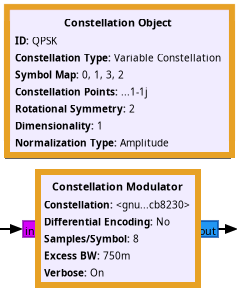
\includegraphics[scale=0.5,valign=c]{img/intro/constellation_mod.png} &\
        \raisebox{7\height}{\minipage[t]{0.65\linewidth-2\fboxsep-2\fboxrule\relax}
            No âmbito da modulaç\~ao em ambiente \textit{GNU Radio}:
            \\[0.2em]
            \hspace*{1em} "(...) The input is a byte stream (unsigned char) and the output is the complex modulated signal at baseband."\cite{constellationmodulator-gnuradio}
            \\[0.2em]
            \hspace*{1em} Pelo que o \textit{output} (que representa o sinal de banda-passante teórico em banda-base) proveniente do bloco \textit{Constellation Modulator} toma o seguinte formato\footnotemark[3]:
            $$ z(t) = I(t)+jQ(t) $$
        \endminipage}
    \end{tabular}
\end{table}

\footnotetext[3]{"Complex baseband equivalent representation of the real [passband] signal."\cite{mathuranathan_2020}}

\newpage
Pelo que

$$ 
    \sqrt{E_b} = \sqrt{\varepsilon} \delequal \sqrt{I(t)^2 + Q(t)^2} \;\; \land \;\; \theta(t) \delequal tan^{-1} \left( \frac{Q(t)}{I(t)} \right)
$$

Deste modo, a análise do sinal é passível de uma abordagem vetorial, como explicitado nos \hyperref[fig:constellations]{\textbf{diagramas de constelação} a baixo}:

\begin{figure}[H]
    \centering
    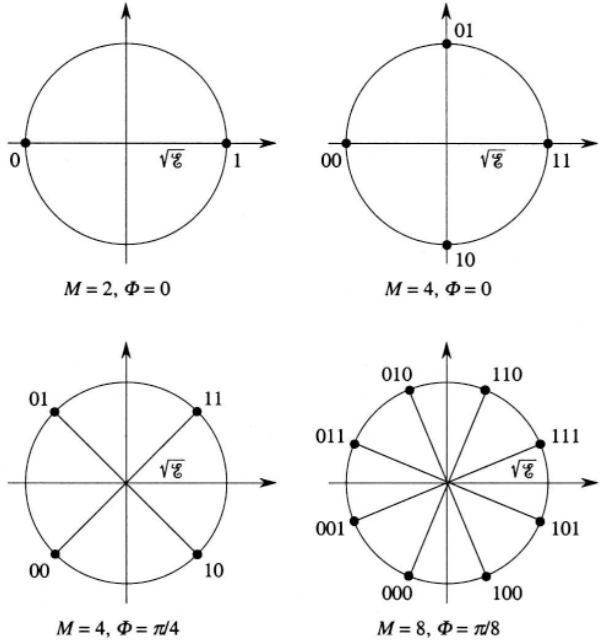
\includegraphics[width = 0.5\linewidth]{img/intro/gray-mapped_constellation.png}
    \caption{Representação geométrica de conjuntos de sinais PSK \textit{Gray-mapped}\cite{benedetto_biglieri_2002}.}
    \label{fig:constellations}
\end{figure}

O mapeamento dos símbolos para a representação em \textit{complex baseband} é garantido no bloco \textit{Constellation Object}. Atendendo ao parâmetro \textit{Variable Constellation}, para um ajuste fino, revela-se:
\begin{itemize}
    \item[] \underline{\textbf{Forma geral:}} \textit{Symbol Map} $\mapsto$ \textit{Constellation Points}
    \item[$\star$] \textbf{BPSK:} $[0, 1]\mapsto[-1, 1]$
    \item[$\star$] \textbf{QPSK:} $[0, 1, 3, 2]\mapsto[\underbrace{-1-1j}_{00},\underbrace{-1+1j}_{01},\underbrace{1+1j}_{11},\underbrace{1-1j}_{10}]$
\end{itemize}
%
%=============================--C--=============================%
\clearpage
\subsection{2. Canal de transmiss\~ao e filtro adaptado}
\label{subsec:filtro-adaptado}
Numa situação ideal (i.e., na ausência de ruído branco), a desmodulação de um sinal digital requer a utilização de um filtro passa-baixo regular. Não obstante, em aplicações reais é necessário mitigar os efeitos da presença do ruído branco (térmico), cuja densidade espectral de potência é constante ($S_W(f)=N_0/2$). Esta característica torna o AWGN impossível de eliminar completamente. 
\\[-7em]

\begin{tabular}{C{6.5cm}  L{6.5cm}}
    \label{fig:gnuradio1}
    \raisebox{-2.1\height}{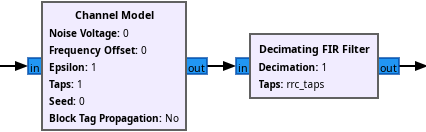
\includegraphics[width = 1\linewidth]{img/intro/channel_matchedfilter.png}}\captionof{figure}{Modelo do canal de transmissão e filtro adaptado (\textit{GNU Radio}).} & \noindent\fcolorbox{black}{white}{%
        \minipage[t]{\dimexpr\linewidth-2\fboxsep-2\fboxrule\relax}
            \textbf{Nota} $\rightarrow$ Em regime laboratorial, o canal de transmiss\~ao é simulado através do bloco \textit{Channel Model}, onde é variado o \textit{"AWGN noise level as a voltage"}\cite{channelmodel-gnuradio} de 0 a 4 V.
        \endminipage}
\end{tabular} 

Para atenuar o impacto deste ruído, utiliza-se um filtro adaptado que maximiza a relação sinal-ruído nos instantes de amostragem.

\begin{figure}[H]
    \centering
    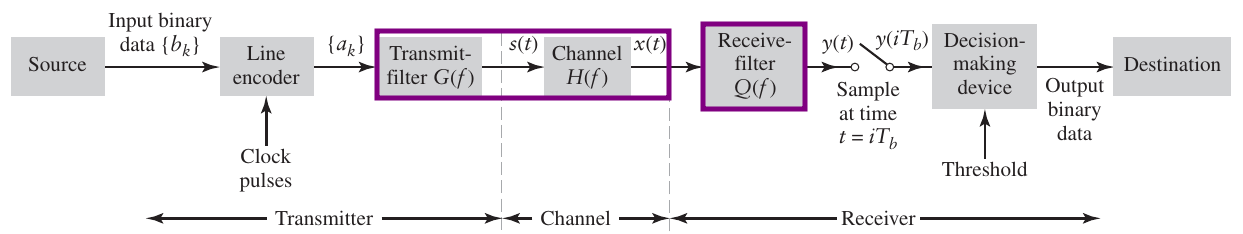
\includegraphics[width = 1\linewidth]{img/intro/filtro_adaptado1.png}
    \caption{Trasmissão e recepção com filtro adaptado.}
    \label{fig:filtro-adaptado}
\end{figure}

Tomando $G(f)H(f) \delequal P^{1/2}(f)$, temos que o filtro adaptado toma a seguinte forma: $Q(f) \delequal P^{1/2}(f)$.\footnotemark[4]

\footnotetext[4]{Sendo o sistema caracterizado por $p(t) = g(t)\ast h(t)\ast q(t) \xrightarrow{\mathcal{F}} P(f) = G(f)H(f)Q(f)$, obtém-se o sinal PAM: $y(t) = \sum\limits_{k=-\infty}^{\infty} a_k p(t-kT_b)$.}

\subsubsection{2.1 \textit{Pulse-shaping}}

\begin{quotation}
    "The most popular pulse-shaping filter seems to be the “raised-cosine” filter. It’s a good low-pass filter for limiting the bandwidth our signal will occupy, and it also has the property of summing to zero at intervals of $T_S$ [eliminar interferência intersimbólica (IIS)] (...)"\cite{pysdr}
\end{quotation}

Mediante o supracitado, e tendo em consideração o formato do sinal $y(t)$ (vide a \hyperref[fig:filtro-adaptado]{Fig. 3}), é trivialmente deduzido que para obter o formato \textit{raised cosine} e executar o processo de \textit{matched filtering} no ramo de receção (tal como no projeto corrente), recorre-se a um \textit{root raised cosine} (como apresentado na \hyperref[fig:gnuradio1]{Fig. 2}).
%
%=============================--C--=============================%
\clearpage
\subsection{3. Desmodulaç\~ao}
No que consta à desmodulação, o processo é efetuado em dois instantes: sincronização de símbolo (efetuada no bloco \textit{Symbol Sync}) e reconversão para stream de dados binários (\textit{Binary Slicer}).

\subsubsection{3.1 \textit{Symbol Sync}}
\label{subsubsec:symbol-sync}
\begin{quote}
    "Symbol timing synchronization has a unique purpose: to find the optimal instants when downsampling a sequence of samples into a series of symbols. In other words, it focuses on selecting the “best” sample out of every group of samples, such that this selected sample can better represent the transmitted symbol. The chosen sample (deemed as the symbol) is then passed on to the symbol detector."\cite{igor}
\end{quote}

\begin{figure}[H]
    \centering
    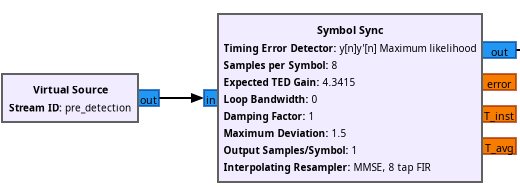
\includegraphics[width = 0.6\linewidth]{img/intro/demod1_symbolsync.png}
    \caption{Bloco que realiza a sincronização de símbolo.}
    \label{fig:symbolsync}
\end{figure}

Concentramos a nossa atenção sobre os seguintes parâmetros: 

\begin{table}[h]
    \centering
    %\setlength{\extrarowheight}{1em}
    \begin{tabular}{l l}
        \minipage[t]{0.5\linewidth-2\fboxsep-2\fboxrule\relax}
            \textbf{\textit{Loop Bandwidth:}}\newline
            "It should nominally be close to 0, but greater than 0. If unsure, start with a number around 2*pi*0.04, and experiment to find the value that works best for your situation."\cite{symbolsync-gnuradio}
        \endminipage &\
        \minipage[t]{0.5\linewidth-2\fboxsep-2\fboxrule\relax}
            \textbf{\textit{TED Gain:}}\newline
            "This value is normally computed by the user analytically or by simulation in a tool outside of GNURadio. This value must be correct for the loop filter gains to be computed properly from the desired input loop bandwidth (...)"\cite{symbolsync-gnuradio}
        \endminipage
    \end{tabular}
\end{table}
\vspace{-1.5em}
\paragraph{3.1.1 \textit{TED (Timing Error Detector)}}\mbox{}\\
\label{subsubsubsec:loopbandwidth}
Tal como supracitado, o bloco \textit{Symbol Sync} requer a computação do \textit{TED Gain} fora do ambiente \textit{GNU Radio} para um correto funcionamento face à \textit{Loop Bandwidth}.

\begin{quote}
"(...) The timing offset error $\tau$ results from the channel propagation delay, which can not be controlled and, therefore, introduces delays that are not simply integer multiples of the symbol period. In reality, the propagation delay is such that $\tau$ is composed of two terms: an integer and a fractional multiple of $T_s$. In the context of symbol timing recovery, we are only concerned with the fractional error. The integer error is handled by a frame timing recovery (or frame synchronization) scheme.

(...) The timing error detector has the purpose of estimating this timing error $\tau$, so that the receiver can adjust its timing and avoid the intersymbol interference."\cite{igor}
\end{quote}

Este breve reparo relativamente ao \textit{Timing Error Detector} salienta a proeminência da correta parametrização deste campo.

\begin{figure}[ht]
    \centering
    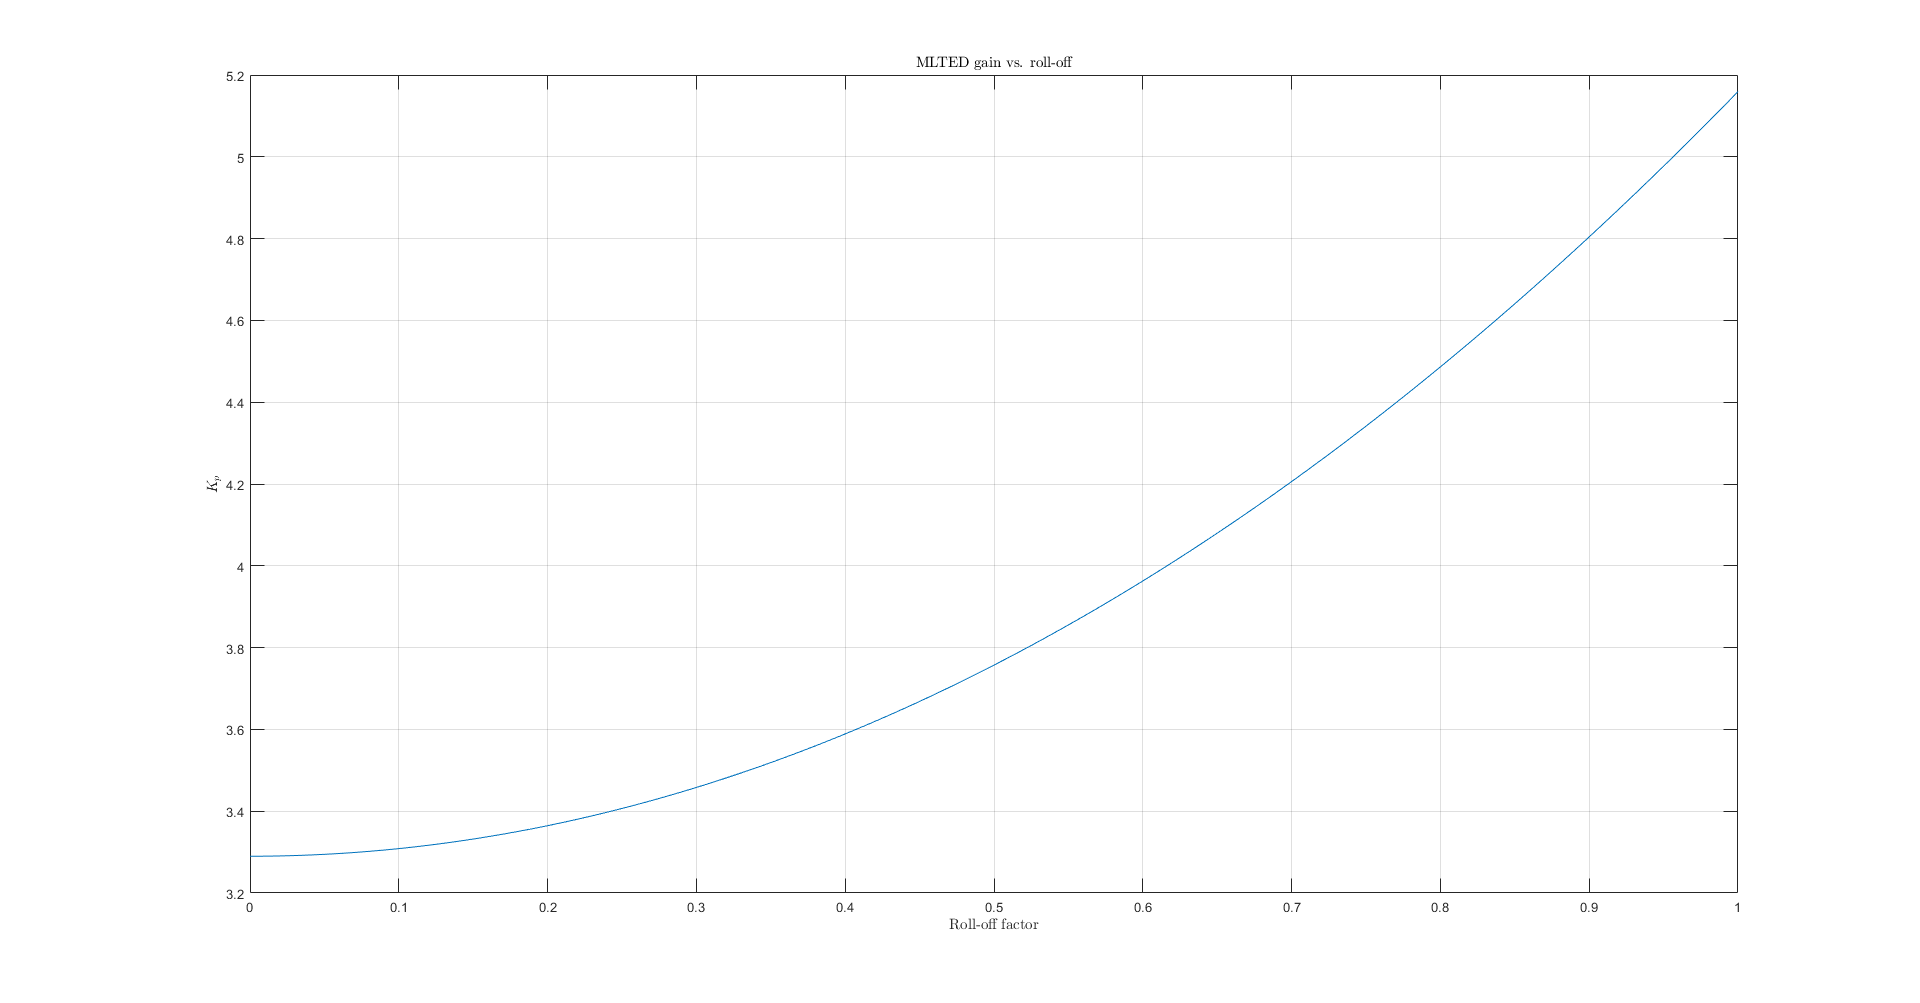
\includegraphics[width=0.85\linewidth]{img/intro/MLTEDgain.png}
    \caption{Evolução do \textit{TED Gain} face ao aumento do \textit{roll-off factor} (MLTED)\cite{igor}.} 
    \label{fig:TEDGain} 
\end{figure} 

O cálculo do ganho é dependente do \textit{roll-off factor} do \textit{root raised cosine} e do esquema do \textit{Timing Error Detector} utilizado (\textit{Maximum Likelihood}). Tal evolução é aparente na \hyperref[fig:TEDGain]{Fig. 5}. Para o \textit{roll-off factor} de $0.75$ especificado no Guia de Laboratório, o valor ótimo calculado\footnotemark[5] para o \textit{TED Gain} verificou-se $4.3415$. A aplicação deste fator é aparente na \hyperref[fig:TEDGain-effect]{Fig. 6}.

\footnotetext[5]{Através do cálculo analítico da constante, com o recurso ao \textit{script} em MATLAB disponibilizado em \href{https://github.com/igorauad/symbol_timing_sync}{https://github.com/igorauad/symbol\_timing\_sync}.}

\begin{figure}[ht]
    \centering
    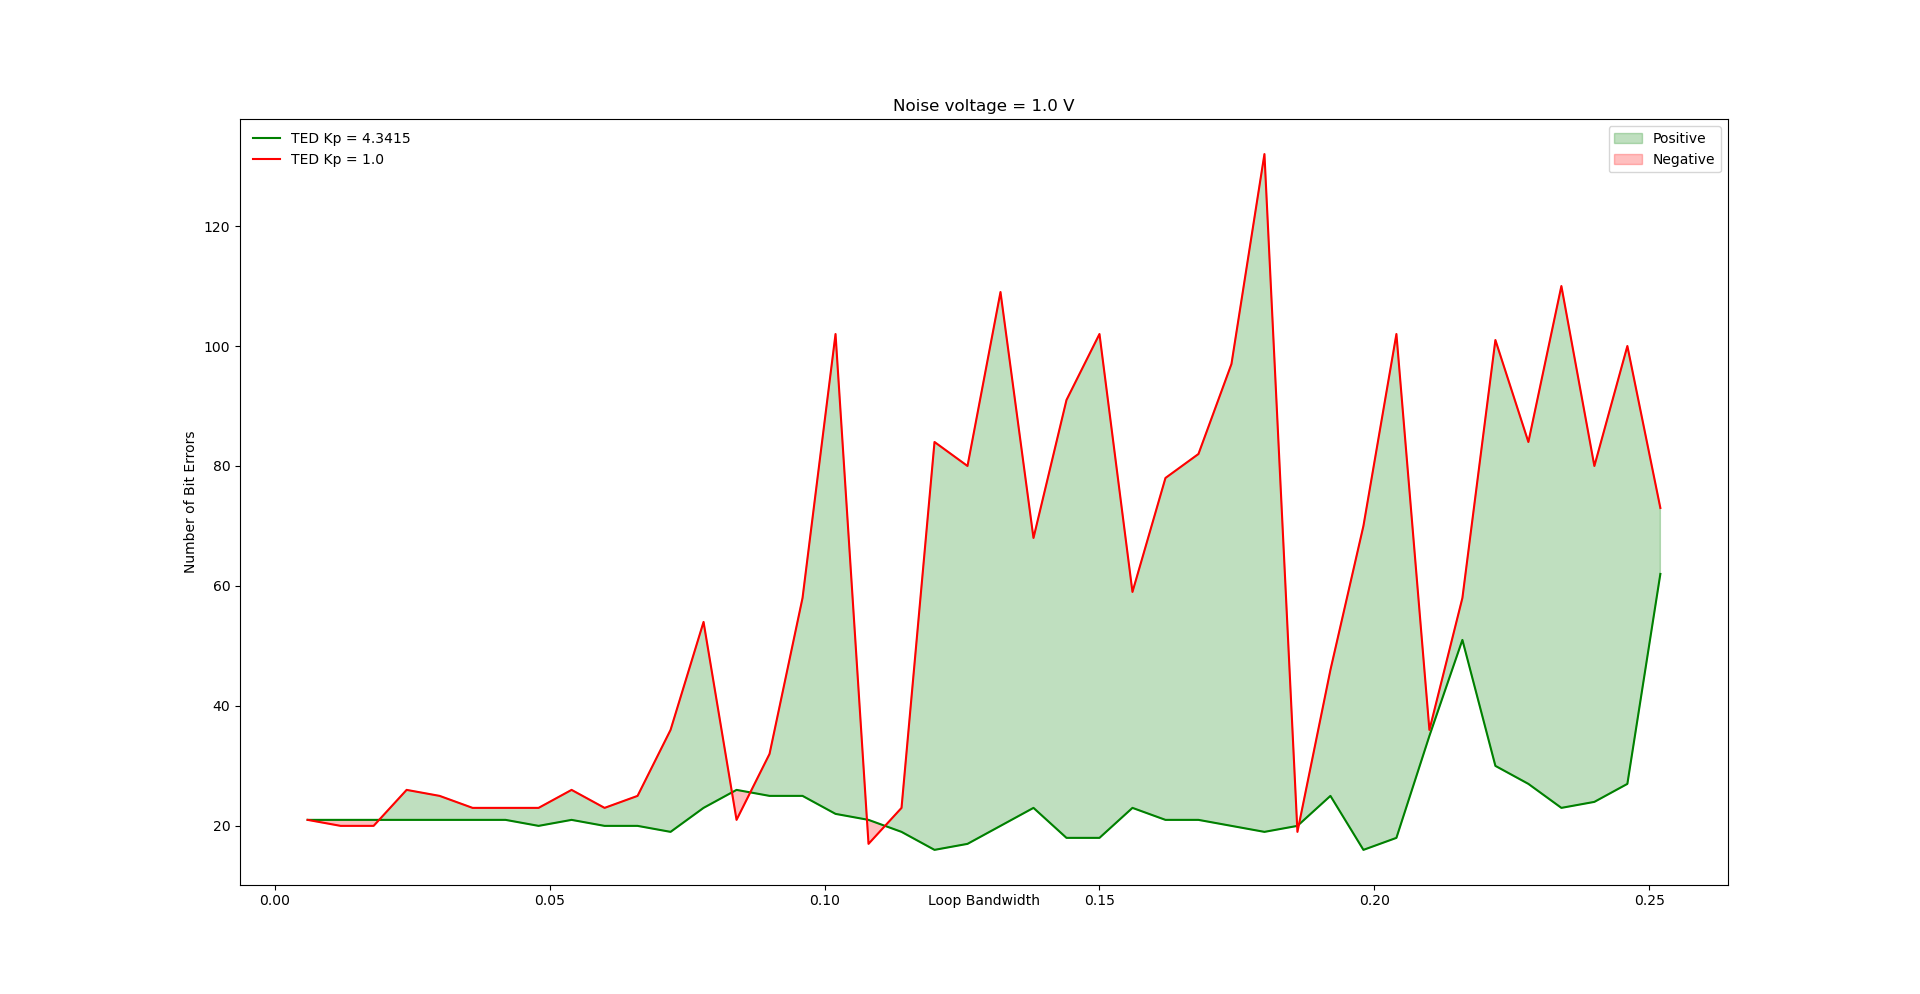
\includegraphics[width=0.85\linewidth]{img/intro/TEDGain_effect.png} 
    \caption{Efeitos da aplicação do \textit{TED Gain} calculado para uma \textit{noise voltage} de 1.0 V.} 
    \label{fig:TEDGain-effect} 
\end{figure} 

A maior estabilidade \hyperref[fig:TEDGain-effect]{observada} para o \textit{range} de valores de \textit{Loop Bandwidth} relevantes para a análise\cite{symbolsync-gnuradio}, é também acompanhada por uma desejável mitigação aparente de erros de bit\footnotemark[6]. Em virtude das ilações expostas, as posteriores simulações são, naturalmente, \textbf{realizadas com um \textit{TED Gain} de 4.3415}.

\footnotetext[6]{Reparos especialmente prevalentes para \textit{Loop Bandwidths} nominalmente perto de zero.}

\clearpage
\paragraph{3.1.2 \textit{Loop Bandwidth}}\mbox{}\\
A função do \textit{Loop Filter} encontrado na composição do bloco \textit{Symbol Sync} (\href{https://wiki.gnuradio.org/index.php/Symbol_Sync}{vide a documentação oficial}) pode ser sucintamente descrita pela seguinte citação:
\begin{quote}
    "\textbf{The loop filter controls how fast the timing error can be corrected, what types of errors can be treated, and the range of correctable timing errors.} In general, it is a second-order system and often the proportional-plus-integral controller (PI controller), commonly used in feedback systems. (...)"\cite{igor}
\end{quote}

O funcionamento deste integrante do processo de sincronizaç\~ao de símbolo é profundamente caracterizado pela sua \textit{Loop Bandwidth}, que:

\begin{quote}
    "(...) sets the boundary at which your recovery loop will track timing noise (jitter/phase noise) in your signal. \textbf{Timing noise has components at all frequencies} (...), and the lower frequency components of the timing noise (...) will be tracked by the timing loop, and therefore suppressed. However the higher frequency components will not be tracked by the timing loop and therefore remain and contribute to noise as part of SNR. \textbf{The timing loop can be viewed as a high pass filter on the jitter/phase noise components}, passing the higher frequency components (including the modulation signals) and supressing the lower frequencies at a rate depending on the order of the loop. Thus you see the motivation to make the timing loop as fast as possible in the interest of tracking out as much timing jitter as possible. \textbf{However, some of the signal energy of interest will be part of the "noise" being supressed by the timing loop}; and this can be quantified by understanding the spectral characteristics of the modulation used. \textbf{As the loop BW increases, too much signal energy is also removed}, and thus it is clear how there can be an optimum setting for the Loop BW that maximizes SNR."\cite{avi1987}
\end{quote}

Procuramos ent\~ao um valor de \textit{Loop Bandwidth} que n\~ao reduza (de forma comprometedora) a relaç\~ao sinal-ruído, mas que suprima as componentes de baixa e alta frequência do \textit{timing noise}. 

\vskip 1em
\noindent\fcolorbox{black}{white}{%
        \minipage[t]{\dimexpr\linewidth-2\fboxsep-2\fboxrule\relax}
            \textbf{Observação} $\rightarrow$ Em regime laboratorial, verifica-se geralmente o supracitado: o número de erros de bit tende\footnotemark[7] a aumentar consoante o incremento após certos \textit{thresholds} da \textit{Loop Bandwidth}, para cada patamar de ruído.
        \endminipage}

\footnotetext[7]{Relação aparente na análise posterior dos dois sistemas.}
%
%=============================--C--=============================%
\subsubsection{3.2 Reconversão para stream de dados binários}
\label{subsubsec:stream-to-bit}
Encontrado o intervalo ótimo de amostragem, ao qual corresponde o valor máximo do pulso, segue-se a conversão para \textit{stream} de dados binários, para a recuperação da sequência de \textit{bits} transmitida.

\clearpage
\paragraph{3.2.1 BPSK}\mbox{}\\
Para clarificar o processo corrente, é relevante apresentar um exemplo prático.

Observando a constelação do \textit{byte} 85 (0 1 0 1 0 1 0 1) repetido \textit{ad eternum}, na ausência dos efeitos do AWGN:
\begin{figure}[H]
    \begin{subfigure}[b]{0.45\linewidth}
        \centering
        \includegraphics[width = 0.8\linewidth]{img/intro/const-byte85-bpsk.png}
        \caption{Constelação do \textit{byte} 85 após a sincronização\\ de símbolo.}
        \label{fig:const-byte85-bpsk}
        \vspace{1ex}
    \end{subfigure}
    \begin{subfigure}[b]{0.45\linewidth}
        \centering
        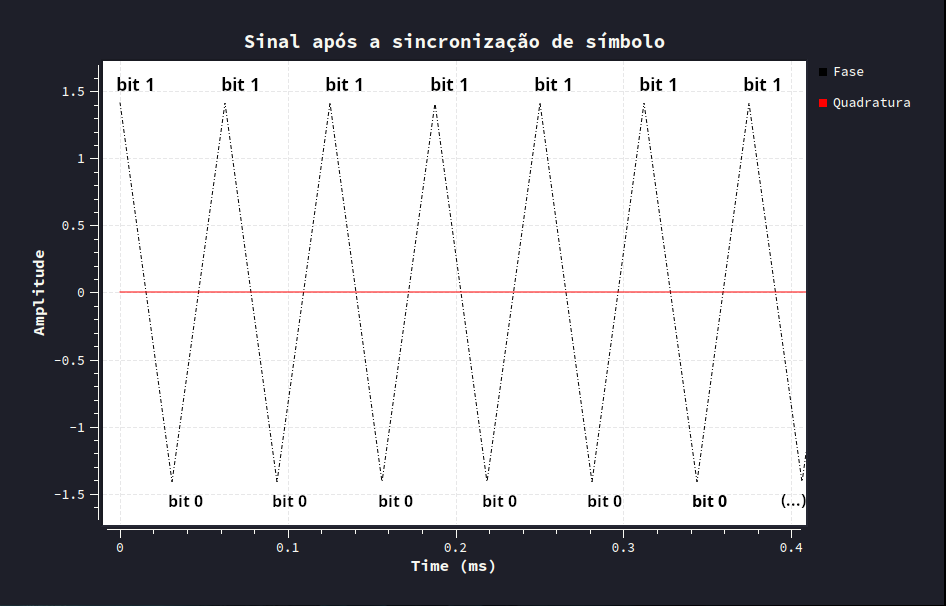
\includegraphics[width = 0.8\linewidth]{img/intro/detected-byte85-bpsk.png}
        \caption{Sinal correspondente ao \textit{byte} 85 após a sincronização de símbolo (sem presença de AWGN).}
        \label{fig:detected-byte85-bpsk}
        \vspace{1ex}
    \end{subfigure}
    \caption{Representações do \textit{byte} 85 numa modulação BPSK (sem normalização\protect\footnotemark[8]).}
\end{figure}
é aparente o mapeamento explicitado na antecedente \hyperref[subsubsec:const-mod]{secção 1.1}:
\vskip -2.5em
\begin{table}[H]
    \centering
    \begin{tabular}{c c}
        \minipage[t]{0.45\linewidth-2\fboxsep-2\fboxrule\relax}
            $$\text{\textit{bit}}\ 1 \mapsto [+1+0j] \xrightarrow[]{} \begin{cases}
                    \text{coef}_{\mathbb{R}\text{e}} = +\sqrt{2}\\
                    \text{coef}_{\mathbb{I}\text{m}} = 0
                \end{cases}
            $$
        \endminipage &\
        \minipage[t]{0.45\linewidth-2\fboxsep-2\fboxrule\relax}
            $$\text{\textit{bit}}\ 0 \mapsto [-1+0j] \xrightarrow[]{} \begin{cases}
                    \text{coef}_{\mathbb{R}\text{e}} = -\sqrt{2}\\
                    \text{coef}_{\mathbb{I}\text{m}} = 0
                \end{cases}
            $$
        \endminipage 
    \end{tabular}
\end{table}

Após a sincronização de símbolo (vide a \hyperref[fig:detected-byte85-bpsk]{Fig. 7} (b)), é apenas necessário recorrer a um bloco decisor para a conversão em \textit{bits} (\textit{Binary Slicer} $\xrightarrow[]{}$ "Positive input produces a binary 1 and negative input produces a binary zero."\cite{binaryslicer-gnuradio}) e efetuar um posterior agrupamento em \textit{bytes} (\textit{Pack K bits}). Tal como apresentado abaixo:

\begin{figure}[H]
    \centering
    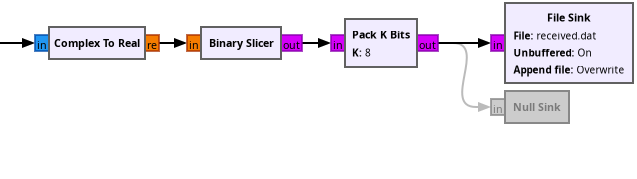
\includegraphics[width = 0.65\linewidth]{img/intro/BPSK_demod.png}
    \caption{Etapa final do processo de desmodulação BPSK em ambiente \textit{GNU Radio}.}
    \label{fig:bpsk-demod}
\end{figure}

\noindent\fcolorbox{black}{white}{%
        \minipage[t]{\dimexpr\linewidth-2\fboxsep-2\fboxrule\relax}
            \textbf{Observação} $\rightarrow$ Em regime laboratorial, verifica-se um \textit{offset} de 49 \textit{bits} no ficheiro ‘received.dat' (ficheiro de saída, vide a \hyperref[fig:bpsk-demod]{Fig. 8}), tal como explicitado no Guia de Laboratório: "(...) De notar que no ficheiro ‘bpsk\_rec.dat', os bits correspondentes aos bits enviados aparecem a partir da 50\textsuperscript{\underline{a}} posição sendo precedidos de 49 bits correspondentes ao buffer interno do módulo ‘Symbol Sync’"\cite{guia_lab}.
        \endminipage}

\footnotetext[8]{Devido a incongruências observadas em diversas plataformas (Windows, GNU/Linux) da opção \textit{Normalization Type} do bloco \hyperref[subsubsec:const-mod]{\textit{Constellation Object}} \cite{constellationobject-gnuradio} em ambiente \textit{GNU Radio}, \textbf{toda a análise subsequente é realizada sem qualquer tipo de normalização} (i.e., $\sqrt{\varepsilon} = \sqrt{2} \neq 1$), de modo a garantir a comparação dos sistemas BPSK e QPSK.}

%---
\clearpage
\paragraph{3.2.2 QPSK}\mbox{}\\
De forma análoga, apresenta-se o exemplo do \textit{byte} 153 (10 01 10 01), em repetição, que nos permite observar a sincronia ortogonal das componentes em fase e em quadratura (característica da modulação QPSK\footnotemark[9]).

\footnotetext[9]{"QPSK can be regarded as a pair of orthogonal BPSK systems, i.e. the real component is one BPSK system, the imaginary component is the second BPSK 
system (...)"\cite{dsp}}

\begin{figure}[H]
    \begin{subfigure}[b]{0.45\linewidth}
        \centering
        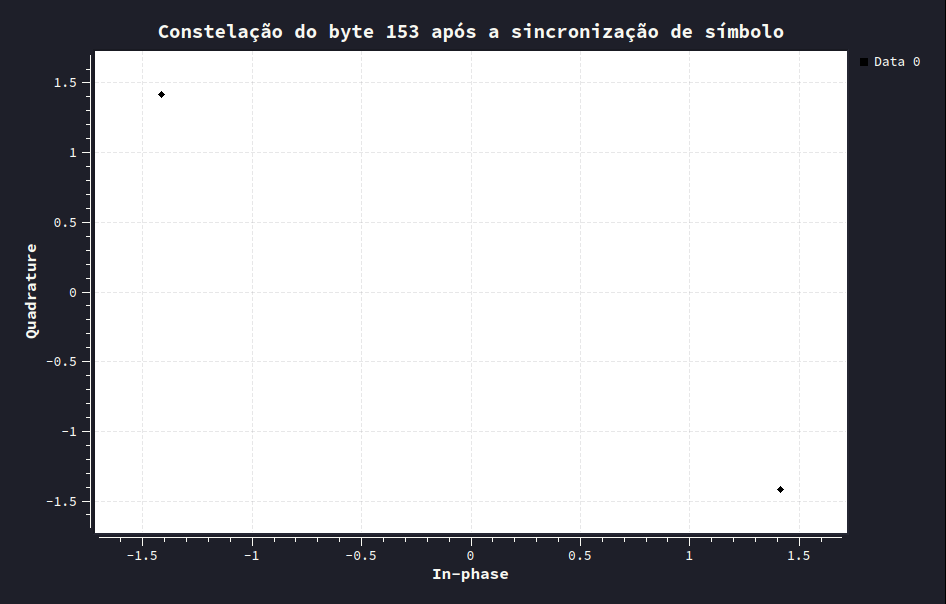
\includegraphics[width = 0.8\linewidth]{img/intro/const-byte153-qpsk.png}
        \caption{Constelação do \textit{byte} 153 após a sincronização\\ de símbolo.}
        \label{fig:const-byte153-qpsk}
        \vspace{1ex}
    \end{subfigure}
    \begin{subfigure}[b]{0.45\linewidth}
        \centering
        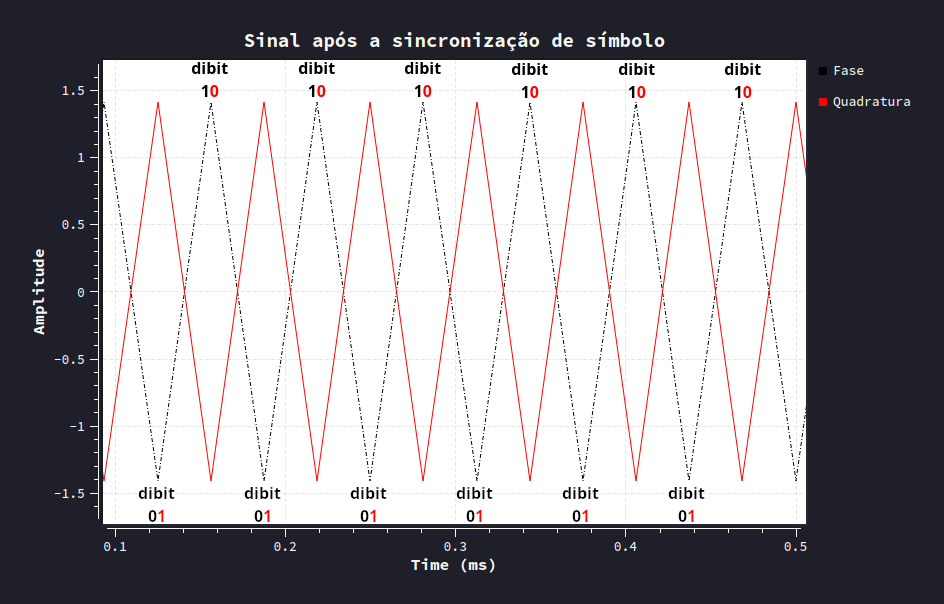
\includegraphics[width = 0.8\linewidth]{img/intro/detected-byte153-qpsk.png}
        \caption{Sinal correspondente ao \textit{byte} 153 após a sincronização de símbolo (sem presença de AWGN).}
        \label{fig:detected-byte153-qpsk}
        \vspace{1ex}
    \end{subfigure}
    \caption{Representações do \textit{byte} 153 numa modulação QPSK (sem normalização).}
\end{figure}
Ainda assim, graças à particularidade referida acima (e na anterior \hyperref[subsubsec:const-mod]{secção 1.1}), um \textit{byte} seccionado em \textit{dibits} pode ser mapeado (de forma ótima, sem AWGN) para as quatro regiões do diagrama de constelação, como se apresenta:

\vskip -2.5em
\begin{table}[h]
    \centering
    \begin{tabular}{l l}
        \minipage[t]{0.5\linewidth-2\fboxsep-2\fboxrule\relax}
            $$
            \begin{tabular}{c}
                \textit{dibit}\\
                11
                \end{tabular} \mkern-9mu\mapsto [+1+1j] \xrightarrow[]{} \begin{cases}
                    \text{coef}_{\mathbb{R}\text{e}} = +\sqrt{2}/2\\
                    \text{coef}_{\mathbb{I}\text{m}} = +\sqrt{2}/2
                \end{cases}
            $$
        \endminipage &\
        \minipage[t]{0.5\linewidth-2\fboxsep-2\fboxrule\relax}
            $$
            \begin{tabular}{c}
                \textit{dibit}\\
                01
                \end{tabular} \mkern-9mu\mapsto [-1+1j] \xrightarrow[]{} \begin{cases}
                    \text{coef}_{\mathbb{R}\text{e}} = -\sqrt{2}/2\\
                    \text{coef}_{\mathbb{I}\text{m}} = +\sqrt{2}/2
                \end{cases}
            $$
        \endminipage \\ 
        \minipage[t]{0.5\linewidth-2\fboxsep-2\fboxrule\relax}
            $$
            \begin{tabular}{c}
                \textit{dibit}\\
                00
                \end{tabular} \mkern-9mu\mapsto [-1-1j] \xrightarrow[]{} \begin{cases}
                    \text{coef}_{\mathbb{R}\text{e}} = -\sqrt{2}/2\\
                    \text{coef}_{\mathbb{I}\text{m}} = -\sqrt{2}/2
                \end{cases}
            $$
        \endminipage &\ 
        \minipage[t]{0.5\linewidth-2\fboxsep-2\fboxrule\relax}
            $$
            \begin{tabular}{c}
                \textit{dibit}\\
                10
                \end{tabular} \mkern-9mu\mapsto [+1-1j] \xrightarrow[]{} \begin{cases}
                    \text{coef}_{\mathbb{R}\text{e}} = +\sqrt{2}/2\\
                    \text{coef}_{\mathbb{I}\text{m}} = -\sqrt{2}/2
                \end{cases}
            $$
        \endminipage
    \end{tabular}
\end{table}

Novamente, após este processo de deteção, segue-se a conversão para \textit{stream} de dados binários, empacotados posteriormente em \textit{bytes}. Este processo assemelha-se ao do BPSK, com a exceção da intercalação das componentes em fase (\textit{bit} mais significativo do \textit{dibit}) e em quadratura (\textit{bit} menos significativo do \textit{dibit}).  

\begin{figure}[H]
    \centering
    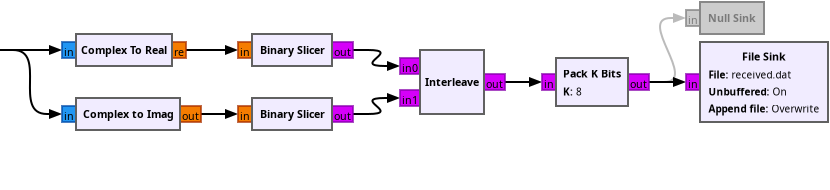
\includegraphics[width = 0.85\linewidth]{img/intro/QPSK_demod.png}
    \caption{Etapa final do processo de desmodulação QPSK em ambiente \textit{GNU Radio}.}
    \label{fig:qpsk-demod}
\end{figure}

\noindent\fcolorbox{black}{white}{%
        \minipage[t]{\dimexpr\linewidth-2\fboxsep-2\fboxrule\relax}
            \textbf{Nota} $\rightarrow$ Verifica-se uma duplicação do \textit{offset} (proveniente do \textit{buffer} do \textit{Symbol Sync}) incutido no ficheiro de saída, (fenómeno esperado) visto que decorrem duas sincronizações em paralelo\footnotemark[9] posteriormente intercaladas. 
        \endminipage}
%
%=============================--D--=============================%
\clearpage
\subsection{4. Probabilidade de erro do bit}
%A ideia do projeto é criarmos um emissor (modulador) que envia um conjunto de bits e sermos capazes com o nosso recetor descodificar a mensagem enviada. 
%Idealmente, na ausência de ruído branco, a sequência de bits descodificados no recetor seria exatamente iguais à transmitida, mas numa situação real existem sempre bits que são erroneamente detetados no seio do ruído.%

Antes de proceder para as etapas de tratamento de dados subsequentes é fundamental analisar a métrica "probabilidade de erro de bit", $P_e$, com vista a fornecer uma preâmbulo à exposição e análise de resultados. Invocando o Teorema da Probabilidade Total e supondo a equiprobabilidade dos bits `1' e `0', a probabilidade de erro será dada por:

\begin{equation*}
    P_e= P(\text{erro}\ |\ \text{bit 1}) P(\text{bit 1})\ +\ P(\text{erro}\ |\  \text{bit 0})P(\text{bit 0})\
\end{equation*}
\[P_e =\dfrac{P(\text{erro}\ |\ \text{bit 1})\ +\ P(\text{erro}\ |\ \text{bit 0})}{2}\]
%
%=============================--D--=============================%
\subsubsection{4.1 Probabilidade de erro  de bit para um sinal binário polar}
\label{subsubsec:prob-erro}
Reconhecendo que o sinal binário polar\footnotemark[10] (onde se encontram os sinais das modulações em análise) pode ser expresso procedimentalmente sobre a forma $y(t)=\sum_{n=-\infty}^{\infty} a_n p(t-nT)$ de amplitudes $a_n=\pm \text{A}$, após a sincronização de símbolo e encontro do instante de amostragem ideal $T_0$ temos:

\begin{equation*}
    p_k=a_n \cdot p_0=   
    \begin{cases}
        +\text{A} \cdot p(T_0)\text{,} & \text{bit 1}\\
        -\text{A} \cdot p(T_0)\text{,} & \text{bit 0} 
    \end{cases}
\end{equation*}

\begin{center}
     em que $p(t)$ denomina a resposta do sistema transmissão-receção (vide a  \hyperref[subsec:filtro-adaptado]{secção 2.}).\\
\end{center}


Podemos então determinar as probabilidades de erro condicionadas:
\vskip -1em
$$
\begin{tabular}{c}
$
    \begin{cases}
        P(\text{erro}\ |\ \text{bit 1}) = P(\text{erro}\ |\ a_n=+A)=P(n_k < -A\cdot p(T_0))\\
        P(\text{erro}\ |\ \text{bit 0})=P(\text{erro}\ |\ a_n=-A)=P(n_k > +A\cdot p(T_0))
    \end{cases}
$
\end{tabular}
\mkern-18mu\mkern-9mu \rightarrow Q\left( \dfrac{A \cdot p(T_0)}{\sigma_n} \right)
$$
E subsequentemente concluir que a probabilidade erro de um sinal binário polar é:

\begin{equation*}\label{eq:6}
    P_e=Q\left( \dfrac{A\cdot p(T_0)}{\sigma_n} \right)
\end{equation*}

%\begin{center}
em que $\sigma_n$ é o desvio padrão do ruído no instante de amostragem.   
%\end{center}
Reescrevendo a probabilidade em função da energia de bit obtemos:

\begin{equation*}\label{eq:7}
    P_e=Q\left( \sqrt{\frac{2 E_b}{N_0}} \right)
\end{equation*}
que é válida para ambas as modulações em análise\footnotemark[11].
\vskip 1em
\noindent\fcolorbox{black}{white}{%
        \minipage[t]{\dimexpr\linewidth-2\fboxsep-2\fboxrule\relax}
            \textbf{Nota} $\rightarrow$ Embora coerente para a probabilidade de erro de bit, o mesmo não acontece para a probabilidade de erro de símbolo: $P_\text{es} \approx \text{log}_2(M) P_e$, admitindo um M = 4 para QPSK e M = 2 para BPSK (\hyperref[subsec:intro]{M-PSK}), observamos que:
            \vskip -1em
            $$
                P_{es\_\text{QPSK}} \approx 2P_{es\_\text{BPSK}}
            $$
        \endminipage}

\footnotetext[10]{Sinal à saída do filtro adaptado, vide \hyperref[subsec:filtro-adaptado]{secção 2}.}
\footnotetext[11]{"QPSK can be regarded as a pair of orthogonal BPSK systems (...)  Because they are orthogonal, they don't interfere (to a good approximation), hence the BER curves are largely equivalent."\cite{dsp}}
    \newpage
%=============================--A--=============================%
\renewcommand{\thefigure}{E\arabic{figure}}
\renewcommand{\thetable}{E\arabic{table}}
\setcounter{figure}{0}
\section{Exposição de dados}
\subsection{E.1 Método de obtenção de dados}

A extração de dados foi realizada primariamente com recurso a dois \textit{scripts} desenvolvidos em \textit{Python}:
\vskip -0.25em
\begin{lstlisting}[caption=\textit{Source code}: \color{white}{\underline{\textit{Script} responsável pela comparação de ficheiros} (bit\_error.py)}, frame=tlrb]{saucecode1}
#!/bin/python3
def bit_error(B):
    file_s = "sent.dat";
    file_r = "received.dat";
    
    if B:
        OFFSET = 49;
    else:
        OFFSET = 49*2;

    SIZE = 27*8;
    bit_errors = 0;
    sent = ""; received = "";
#-----
    read_s = open(file_s,'rb').read(); 
    read_r = open(file_r,'rb').read(); 

    for s in read_s:
        sent += '{0:08b}'.format(s);
    for r in read_r:
        received += '{0:08b}'.format(r);

    for i in range(0, SIZE):
        #print((sent[i], received[i+OFFSET]))
        if(sent[i] != received[i+OFFSET]):
            bit_errors += 1;

    print("SENT: \n" + sent[:SIZE] + "\n")
    print("RECEIVED: \n" + received[OFFSET:OFFSET+SIZE])

    print("Bit errors: " + str(bit_errors));
    return bit_errors

\end{lstlisting}
\vskip -0.75em
\begin{lstlisting}[caption=\textit{Source code}: \color{white}{\underline{\textit{Script} responsável pela automatização da comparação de ficheiros} (sim.py)}, frame=tlrb]{saucecode2}
#!/bin/python3
import signal
from bit_error import bit_error 

B=True;
BW = 0.0; N = 0.0;

if B:
    from mdBPSK_copy import mdBPSK as top_block_cls
else:
    from mdQPSK_copy import mdQPSK as top_block_cls

#-----
def sim():
    N0 = [x/2 for x in range(9)];
    loop_BW = [round(6/100 * x/10, 3) for x in range(1,43)];
    #---
    f = open("data.csv", "w"); f.write("N,BW,bit_errors\n")
    #--- .csv
    for N in N0:
        for BW in loop_BW:
            tb = top_block_cls(BW,N); #simulação
            tb.start();
            #tb.show();
            tb.wait();
            b = bit_error(B);
            f.write(str(N) + "," + str(BW) + "," + str(b) + "\n");

    tb.show();
    #---
    f.close();
    #---
    def sig_handler(sig=None, frame=None):
        tb.stop();
        tb.wait();
    #---
    signal.signal(signal.SIGINT, sig_handler);
    signal.signal(signal.SIGTERM, sig_handler);
\end{lstlisting}

As alterações necessárias foram aplicadas aos ficheiros \textit{Python} criados de forma automática pelo \textit{software} \textit{GNU Radio} de modo a que se tornassem suscetíveis à automatização requerida para a análise de dados significantes subsequente.

\label{sec:analise}
%=============================--A--=============================%
%\definecolor{green}{rgb}{0.1,0.1,0.1}
\subsection{E.2 Análise do sistema BPSK}
\label{sec:analiseBPSK}
\vskip -0.5em
\begin{table}[H]
\caption{Taxa de erro de \textit{bit} em função da \textit{Loop Bandwidth}, para cada \textit{noise voltage}.}
\vskip -0.5em
\label{tab:bpsk}
\hspace*{-0.75cm}\begin{tabular}{|c|c|c|c|c|c|c|c|c|c|}
\hline
Loop BW/Noise & 0.0 & 0.5 & 1.0 & 1.5 & 2.0 & 2.5 & 3.0 & 3.5 & 4.0 \\
\hline\hline
0.006 &\cellcolor{green!25}0.0\% & 1.4\% & 9.7\% & 19.0\% & 25.5\% & 30.6\% & 34.7\% & 38.0\% & 39.4\% \\
\hline
0.012 &\cellcolor{green!25}0.0\% & 1.4\% & 9.7\% & 19.0\% & 25.0\% & 29.6\% & 34.3\% & 35.6\% & 38.0\% \\
\hline
0.018 &\cellcolor{green!25}0.0\% & 1.4\% & 9.7\% & 19.4\% & 25.0\% & 28.7\% & 33.3\% & 36.6\% & \cellcolor{green!25}33.8\% \\
\hline
0.024 &\cellcolor{green!25}0.0\% & 1.4\% & 9.7\% & 19.4\% & \cellcolor{green!25}24.5\% & 29.6\% & 34.7\% & 39.4\% & 34.3\% \\
\hline
0.03 &\cellcolor{green!25}0.0\% & 1.4\% & 9.7\% & 19.0\% & \cellcolor{green!25}24.5\% & 29.6\% & 34.7\% & 34.3\% & 37.5\% \\
\hline
0.036 &\cellcolor{green!25}0.0\% & 1.4\% & 9.7\% & 19.0\% & 25.0\% & 28.7\% & \cellcolor{green!25}31.0\% & \cellcolor{green!25}33.3\% & 38.9\% \\
\hline
0.042 &\cellcolor{green!25}0.0\% & 1.4\% & 9.7\% & 18.5\% & 25.0\% & 37.0\% & 32.4\% & 34.3\% & 39.8\% \\
\hline
0.048 &\cellcolor{green!25}0.0\% & 1.4\% & 9.3\% & 18.5\% & \cellcolor{green!25}24.5\% & \cellcolor{green!25}28.2\% & \cellcolor{green!25}31.0\% & 36.1\% & 44.9\% \\
\hline
0.054 &\cellcolor{green!25}0.0\% &\cellcolor{green!25}0.9\% & 9.7\% & 18.5\% & 35.2\% & 31.5\% & \cellcolor{green!25}31.0\% & 38.0\% & 39.4\% \\
\hline
0.06 &\cellcolor{green!25}0.0\% &\cellcolor{green!25}0.9\% & 9.3\% & 20.8\% & 25.0\% & 28.7\% & 34.7\% & 50.0\% & 43.1\% \\
\hline
0.066 &\cellcolor{green!25}0.0\% &\cellcolor{green!25}0.9\% & 9.3\% & 20.4\% & 25.0\% & \cellcolor{green!25}28.2\% & 34.7\% & 40.3\% & 41.2\% \\
\hline
0.072 &\cellcolor{green!25}0.0\% &\cellcolor{green!25}0.9\% & 8.8\% & 19.9\% & 25.9\% & 27.3\% & 33.3\% & 56.0\% & 55.1\% \\
\hline
0.078 &\cellcolor{green!25}0.0\% &\cellcolor{green!25}0.9\% & 10.6\% & 19.0\% & 27.3\% & 29.2\% & 40.7\% & 40.3\% & 44.4\% \\
\hline
0.084 &\cellcolor{green!25}0.0\% &\cellcolor{green!25}0.9\% & 12.0\% & 19.4\% & 26.9\% & 29.6\% & 37.5\% & 35.6\% & 42.6\% \\
\hline
0.09 &\cellcolor{green!25}0.0\% &\cellcolor{green!25}0.9\% & 11.6\% & \cellcolor{green!25}16.7\% & 27.8\% & 38.4\% & 41.2\% & 56.9\% & 51.4\% \\
\hline
0.096 &\cellcolor{green!25}0.0\% &\cellcolor{green!25}0.9\% & 11.6\% & 17.1\% & 25.9\% & 38.4\% & 48.1\% & 32.4\% & 49.5\% \\
\hline
0.102 &\cellcolor{green!25}0.0\% &\cellcolor{green!25}0.9\% & 10.2\% & 19.9\% & 25.5\% & 41.7\% & 44.4\% & 42.1\% & 50.5\% \\
\hline
0.108 &\cellcolor{green!25}0.0\% &\cellcolor{green!25}0.9\% & 9.7\% & 20.4\% & 25.5\% & 38.4\% & 49.1\% & 46.3\% & 54.2\% \\
\hline
0.114 &\cellcolor{green!25}0.0\% &\cellcolor{green!25}0.9\% & 8.8\% & 23.1\% & 30.1\% & 37.0\% & 47.7\% & 42.1\% & 50.0\% \\
\hline
0.12 &\cellcolor{green!25}0.0\% &\cellcolor{green!25}0.9\% & \cellcolor{green!25}7.4\% & 18.5\% & 39.8\% & 44.4\% & 51.9\% & 48.1\% & 49.5\% \\
\hline
0.126 &\cellcolor{green!25}0.0\% &\cellcolor{green!25}0.9\% & 7.9\% & 21.3\% & 40.7\% & 33.3\% & 48.6\% & 47.7\% & 46.3\% \\
\hline
0.132 &\cellcolor{green!25}0.0\% &\cellcolor{green!25}0.9\% & 9.3\% & 19.9\% & 44.0\% & 33.3\% & 47.2\% & 53.7\% & 48.6\% \\
\hline
0.138 &\cellcolor{green!25}0.0\% &\cellcolor{green!25}0.9\% & 10.6\% & 21.8\% & 37.5\% & 37.0\% & 48.1\% & 47.7\% & 50.0\% \\
\hline
0.144 &\cellcolor{green!25}0.0\% &\cellcolor{green!25}0.9\% & 8.3\% & \cellcolor{green!25}16.7\% & 37.5\% & 44.9\% & 50.5\% & 44.0\% & 53.7\% \\
\hline
0.15 &\cellcolor{green!25}0.0\% &\cellcolor{green!25}0.9\% & 8.3\% & 19.0\% & 38.0\% & 39.4\% & 43.1\% & 44.9\% & 53.2\% \\
\hline
0.156 &\cellcolor{green!25}0.0\% &\cellcolor{green!25}0.9\% & 10.6\% & 17.1\% & 28.2\% & 36.1\% & 47.7\% & 53.2\% & 50.5\% \\
\hline
0.162 &\cellcolor{green!25}0.0\% &\cellcolor{green!25}0.9\% & 9.7\% & 19.0\% & 44.0\% & 35.2\% & 44.4\% & 44.4\% & 53.7\% \\
\hline
0.168 &\cellcolor{green!25}0.0\% &\cellcolor{green!25}0.9\% & 9.7\% & 21.8\% & 31.9\% & 48.1\% & 41.7\% & 52.3\% & 51.9\% \\
\hline
0.174 &\cellcolor{green!25}0.0\% &\cellcolor{green!25}0.9\% & 9.3\% & 27.8\% & 39.8\% & 43.1\% & 53.7\% & 50.5\% & 44.4\% \\
\hline
0.18 &\cellcolor{green!25}0.0\% &\cellcolor{green!25}0.9\% & 8.8\% & 31.0\% & 48.6\% & 50.5\% & 45.4\% & 53.2\% & 47.2\% \\
\hline
0.186 &\cellcolor{green!25}0.0\% &\cellcolor{green!25}0.9\% & 9.3\% & 30.6\% & 42.1\% & 44.4\% & 52.3\% & 57.9\% & 46.8\% \\
\hline
0.192 &\cellcolor{green!25}0.0\% &\cellcolor{green!25}0.9\% & 11.6\% & 21.8\% & 48.1\% & 42.6\% & 51.9\% & 52.3\% & 49.5\% \\
\hline
0.198 &\cellcolor{green!25}0.0\% & 1.4\% & \cellcolor{green!25}7.4\% & 21.3\% & 45.8\% & 52.8\% & 45.4\% & 46.8\% & 47.2\% \\
\hline
0.204 &\cellcolor{green!25}0.0\% & 1.4\% & 8.3\% & 39.8\% & 44.4\% & 57.9\% & 51.4\% & 49.1\% & 51.9\% \\
\hline
0.21 &\cellcolor{green!25}0.0\% &\cellcolor{green!25}0.9\% & 16.2\% & 42.6\% & 34.3\% & 30.6\% & 50.5\% & 45.8\% & 50.5\% \\
\hline
0.216 &\cellcolor{green!25}0.0\% & 1.9\% & 23.6\% & 40.7\% & 43.5\% & 40.3\% & 43.5\% & 45.8\% & 50.5\% \\
\hline
0.222 &\cellcolor{green!25}0.0\% & 1.4\% & 13.9\% & 53.2\% & 44.0\% & 53.2\% & 51.9\% & 44.4\% & 50.9\% \\
\hline
0.228 &\cellcolor{green!25}0.0\% & 1.9\% & 12.5\% & 19.9\% & 36.6\% & 48.6\% & 47.2\% & 48.1\% & 49.5\% \\
\hline
0.234 &\cellcolor{green!25}0.0\% & 8.3\% & 10.6\% & 31.9\% & 25.9\% & 47.2\% & 48.6\% & 45.8\% & 54.6\% \\
\hline
0.24 &\cellcolor{green!25}0.0\% &\cellcolor{green!25}0.9\% & 11.1\% & 38.9\% & 36.6\% & 44.9\% & 44.4\% & 50.5\% & 51.9\% \\
\hline
0.246 &\cellcolor{green!25}0.0\% & 1.4\% & 12.5\% & 38.4\% & 46.8\% & 49.1\% & 52.8\% & 50.5\% & 42.1\% \\
\hline
0.252 &\cellcolor{green!25}0.0\% & 1.4\% & 28.7\% & 21.8\% & 49.5\% & 44.9\% & 45.4\% & 43.5\% & 52.3\%\\
\hline
\end{tabular}
\end{table}

%---
\begin{figure}[H]
    \centering
    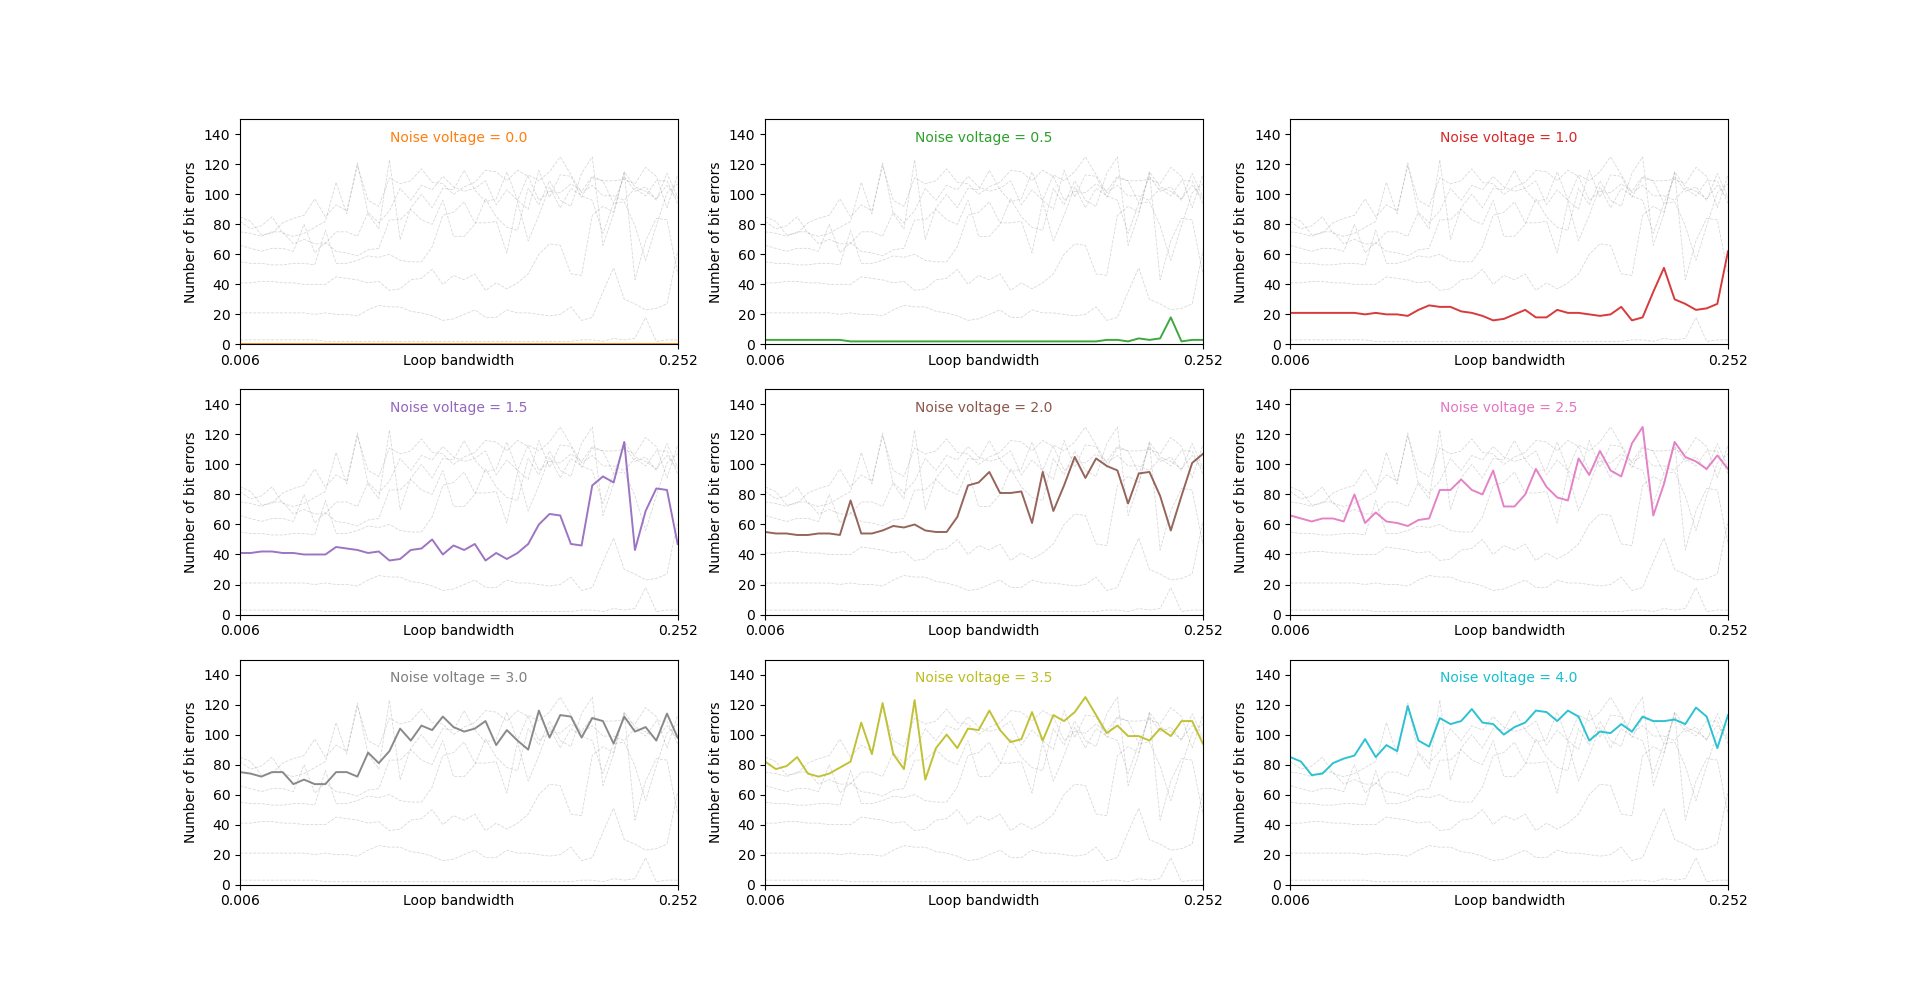
\includegraphics[width=1\linewidth]{img/analise/BPSK_9.png}
    \caption{Evolução do número de erros de \textit{bit} para cada \textit{noise voltage}, em função da \textit{Loop Bandwidth}.}
    \label{fig:bpsk9}
\end{figure}

\noindent\fcolorbox{black}{white}{%
        \minipage[t]{\dimexpr\linewidth-2\fboxsep-2\fboxrule\relax}
            \textbf{Observação 1} $\rightarrow$ Verifica-se, como esperado, um número de erros cada vez mais prevalente e mais oscilante para valores de \textit{Loop Bandwidth} cada vez mais distantes de zero (distanciamento da gama ótima de valores\cite{symbolsync-gnuradio} discutida anteriormente na \hyperref[subsubsec:symbol-sync]{secção 3.1}). É também de salientar a proporcionalidade observada (e expectável) do número de erros de \textit{bit} com o patamar de ruído (aumento da dificuldade em detetar o pulso no seio do ruído $\implies$ maior taxa de erro de \textit{bit}).
        \endminipage}

\vskip 1em
\noindent\fcolorbox{black}{white}{%
        \minipage[t]{\dimexpr\linewidth-2\fboxsep-2\fboxrule\relax}
            \textbf{Observação 2} $\rightarrow$ Para cada gráfico é aparente uma zona de maior estabilidade (número de erros bastante próximos) que tende a contrair e a mutar para uma extensão cada vez mais instável, com o aumento da \textit{noise voltage}. 
        \endminipage}

\vskip 1em
\noindent\fcolorbox{black}{white}{%
        \minipage[t]{\dimexpr\linewidth-2\fboxsep-2\fboxrule\relax}
            \textbf{Nota} $\rightarrow$ Encontram-se a \textcolor{green}{verde} na tabela os valores da \textit{Loop Bandwidth} que minimizam a taxa de erro de \textit{bit} para cada patamar de ruído no sistema BPSK projetado. A segunda observação é corroborada por estes valores \textit{highlighted}, dado que o valor ótimo de \textit{Loop Bandwidth} aparenta tender para valores nominalmente mais próximos de zero com o aumento da \textit{noise voltage}. 
        \endminipage}
%=============================--A--=============================%
\subsection{E.3 Análise do sistema QPSK}
\label{sec:analiseQPSK}
\vskip -0.5em
\begin{table}[H]
\caption{Taxa de erro de \textit{bit} em função da \textit{Loop Bandwidth}, para cada \textit{noise voltage}.}
\vskip -0.5em
\label{tab:qpsk}
\hspace*{-0.75cm}\begin{tabular}{|c|c|c|c|c|c|c|c|c|c|}
\hline
Loop BW/Noise & 0.0 & 0.5 & 1.0 & 1.5 & 2.0 & 2.5 & 3.0 & 3.5 & 4.0 \\
\hline\hline
0.006 & \cellcolor{green!25}0.0\% & 1.9\% & 11.1\% & 19.0\% & 28.2\% & 31.5\% & 34.3\% & 36.6\% & 38.0\% \\
\hline
0.012 & \cellcolor{green!25}0.0\% & 1.4\% & 11.1\% & 19.0\% & 27.8\% & 31.0\% & 33.8\% & 35.6\% & 37.5\% \\
\hline
0.018 & \cellcolor{green!25}0.0\% & 1.4\% & 10.6\% & 18.5\% & 26.4\% & 30.6\% & 33.3\% & 36.6\% & \cellcolor{green!25}32.9\% \\
\hline
0.024 & \cellcolor{green!25}0.0\% & 1.4\% & 10.6\% & 18.1\% & 26.9\% & 29.6\% & 33.3\% & \cellcolor{green!25}32.4\% & 35.2\% \\
\hline
0.03 & \cellcolor{green!25}0.0\% & 1.4\% & 9.7\% & 18.1\% & 25.5\% & 29.6\% & \cellcolor{green!25}31.0\% & 35.2\% & 33.8\% \\
\hline
0.036 & \cellcolor{green!25}0.0\% & 0.5\% & 9.3\% & 17.6\% & 25.0\% & 28.2\% & 35.2\% & 35.6\% & 35.2\% \\
\hline
0.042 & \cellcolor{green!25}0.0\% & 0.5\% & 9.3\% & 17.6\% & \cellcolor{green!25}23.1\% & \cellcolor{green!25}27.3\% & 33.8\% & 33.3\% & 41.7\% \\
\hline
0.048 & \cellcolor{green!25}0.0\% & 0.5\% & 9.7\% & 17.6\% & 25.0\% & 30.1\% & 34.7\% & 32.9\% & 46.8\% \\
\hline
0.054 & \cellcolor{green!25}0.0\% & 0.5\% & 9.3\% & 17.1\% & 24.5\% & 29.6\% & 36.6\% & 41.2\% & 37.0\% \\
\hline
0.06 & \cellcolor{green!25}0.0\% & \cellcolor{green!25}0.0\% & 9.7\% & \cellcolor{green!25}15.7\% & 31.0\% & 30.1\% & 38.0\% & 33.8\% & 45.8\% \\
\hline
0.066 & \cellcolor{green!25}0.0\% & \cellcolor{green!25}0.0\% & 7.9\% & 17.1\% & 24.1\% & 36.1\% & 32.9\% & 44.0\% & 37.5\% \\
\hline
0.072 & \cellcolor{green!25}0.0\% & \cellcolor{green!25}0.0\% & 6.9\% & 19.9\% & 26.4\% & 31.5\% & 54.6\% & 44.0\% & 56.0\% \\
\hline
0.078 & \cellcolor{green!25}0.0\% & \cellcolor{green!25}0.0\% & 8.3\% & 17.6\% & 27.8\% & 41.2\% & 34.7\% & 35.2\% & 50.5\% \\
\hline
0.084 & \cellcolor{green!25}0.0\% & \cellcolor{green!25}0.0\% & 8.3\% & 23.1\% & 27.8\% & 45.4\% & 55.1\% & 34.3\% & 52.8\% \\
\hline
0.09 & \cellcolor{green!25}0.0\% & \cellcolor{green!25}0.0\% & 6.9\% & 22.7\% & 25.9\% & 41.7\% & 45.4\% & 48.1\% & 46.8\% \\
\hline
0.096 & \cellcolor{green!25}0.0\% & \cellcolor{green!25}0.0\% & 8.8\% & 25.9\% & 25.9\% & 31.9\% & 36.1\% & 38.4\% & 46.3\% \\
\hline
0.102 & \cellcolor{green!25}0.0\% & \cellcolor{green!25}0.0\% & 6.5\% & 18.5\% & 48.6\% & 30.6\% & 51.4\% & 49.5\% & 48.6\% \\
\hline
0.108 & \cellcolor{green!25}0.0\% & \cellcolor{green!25}0.0\% & \cellcolor{green!25}2.8\% & 17.6\% & 51.4\% & 40.3\% & 52.8\% & 51.9\% & 43.1\% \\
\hline
0.114 & \cellcolor{green!25}0.0\% & \cellcolor{green!25}0.0\% & 3.7\% & 19.9\% & 48.6\% & 37.5\% & 34.3\% & 53.2\% & 38.9\% \\
\hline
0.12 & \cellcolor{green!25}0.0\% & \cellcolor{green!25}0.0\% & 8.8\% & 33.8\% & 27.3\% & 54.6\% & 49.1\% & 50.9\% & 57.4\% \\
\hline
0.126 & \cellcolor{green!25}0.0\% & \cellcolor{green!25}0.0\% & 10.6\% & 20.4\% & 30.6\% & 50.0\% & 54.6\% & 53.7\% & 46.3\% \\
\hline
0.132 & \cellcolor{green!25}0.0\% & \cellcolor{green!25}0.0\% & 8.8\% & 33.3\% & 26.9\% & 34.7\% & 49.5\% & 52.8\% & 50.5\% \\
\hline
0.138 & \cellcolor{green!25}0.0\% & \cellcolor{green!25}0.0\% & 13.9\% & 16.7\% & 27.8\% & 44.9\% & 51.4\% & 47.7\% & 53.2\% \\
\hline
0.144 & \cellcolor{green!25}0.0\% & \cellcolor{green!25}0.0\% & 17.1\% & 16.2\% & 30.6\% & 47.7\% & 47.2\% & 53.2\% & 57.4\% \\
\hline
0.15 & \cellcolor{green!25}0.0\% & \cellcolor{green!25}0.0\% & 15.3\% & 19.0\% & 26.4\% & 50.9\% & 50.5\% & 50.9\% & 51.9\% \\
\hline
0.156 & \cellcolor{green!25}0.0\% & \cellcolor{green!25}0.0\% & 31.0\% & 49.1\% & 33.8\% & 33.3\% & 49.5\% & 54.2\% & 54.2\% \\
\hline
0.162 & \cellcolor{green!25}0.0\% & \cellcolor{green!25}0.0\% & 15.7\% & 50.9\% & 25.9\% & 41.2\% & 47.2\% & 49.1\% & 52.3\% \\
\hline
0.168 & \cellcolor{green!25}0.0\% & \cellcolor{green!25}0.0\% & 16.2\% & 47.7\% & 25.0\% & 36.1\% & 50.9\% & 52.8\% & 53.7\% \\
\hline
0.174 & \cellcolor{green!25}0.0\% & \cellcolor{green!25}0.0\% & 8.3\% & 39.8\% & 33.3\% & 47.2\% & 47.2\% & 55.6\% & 48.6\% \\
\hline
0.18 & \cellcolor{green!25}0.0\% & \cellcolor{green!25}0.0\% & 6.5\% & 35.2\% & 35.2\% & 32.4\% & 53.7\% & 51.4\% & 45.8\% \\
\hline
0.186 & \cellcolor{green!25}0.0\% & \cellcolor{green!25}0.0\% & 10.2\% & 35.6\% & 31.5\% & 53.7\% & 48.6\% & 42.1\% & 50.9\% \\
\hline
0.192 & \cellcolor{green!25}0.0\% & \cellcolor{green!25}0.0\% & 10.2\% & 21.3\% & 32.4\% & 49.1\% & 56.5\% & 52.8\% & 53.7\% \\
\hline
0.198 & \cellcolor{green!25}0.0\% & \cellcolor{green!25}0.0\% & 29.6\% & 19.4\% & 40.3\% & 53.7\% & 52.8\% & 51.9\% & 53.2\% \\
\hline
0.204 & \cellcolor{green!25}0.0\% & \cellcolor{green!25}0.0\% & 29.2\% & 19.4\% & 43.1\% & 52.8\% & 52.3\% & 45.8\% & 47.2\% \\
\hline
0.21 & \cellcolor{green!25}0.0\% & 0.9\% & 10.6\% & 31.0\% & 50.9\% & 53.7\% & 48.6\% & 50.5\% & 42.6\% \\
\hline
0.216 & \cellcolor{green!25}0.0\% & 0.9\% & 30.1\% & 23.6\% & 43.5\% & 47.2\% & 44.9\% & 50.5\% & 40.3\% \\
\hline
0.222 & \cellcolor{green!25}0.0\% & 0.5\% & 10.2\% & 21.8\% & 31.9\% & 29.2\% & 46.3\% & 48.6\% & 51.4\% \\
\hline
0.228 & \cellcolor{green!25}0.0\% & 0.5\% & 7.4\% & 22.2\% & 36.6\% & 48.1\% & 48.6\% & 49.1\% & 53.7\% \\
\hline
0.234 & \cellcolor{green!25}0.0\% & 0.5\% & 7.9\% & 21.8\% & 32.4\% & 51.4\% & 51.9\% & 50.0\% & 51.4\% \\
\hline
0.24 & \cellcolor{green!25}0.0\% & 0.5\% & 6.0\% & 47.2\% & 38.0\% & 47.7\% & 48.1\% & 44.9\% & 44.9\% \\
\hline
0.246 & \cellcolor{green!25}0.0\% & \cellcolor{green!25}0.0\% & 6.5\% & 48.1\% & 51.9\% & 45.4\% & 47.7\% & 44.0\% & 51.9\% \\
\hline
0.252 & \cellcolor{green!25}0.0\% & 0.5\% & 11.1\% & 50.0\% & 46.3\% & 55.1\% & 54.2\% & 52.3\% & 42.6\% \\
\hline
\end{tabular}
\end{table}

%---
\begin{figure}[H]
    \centering
    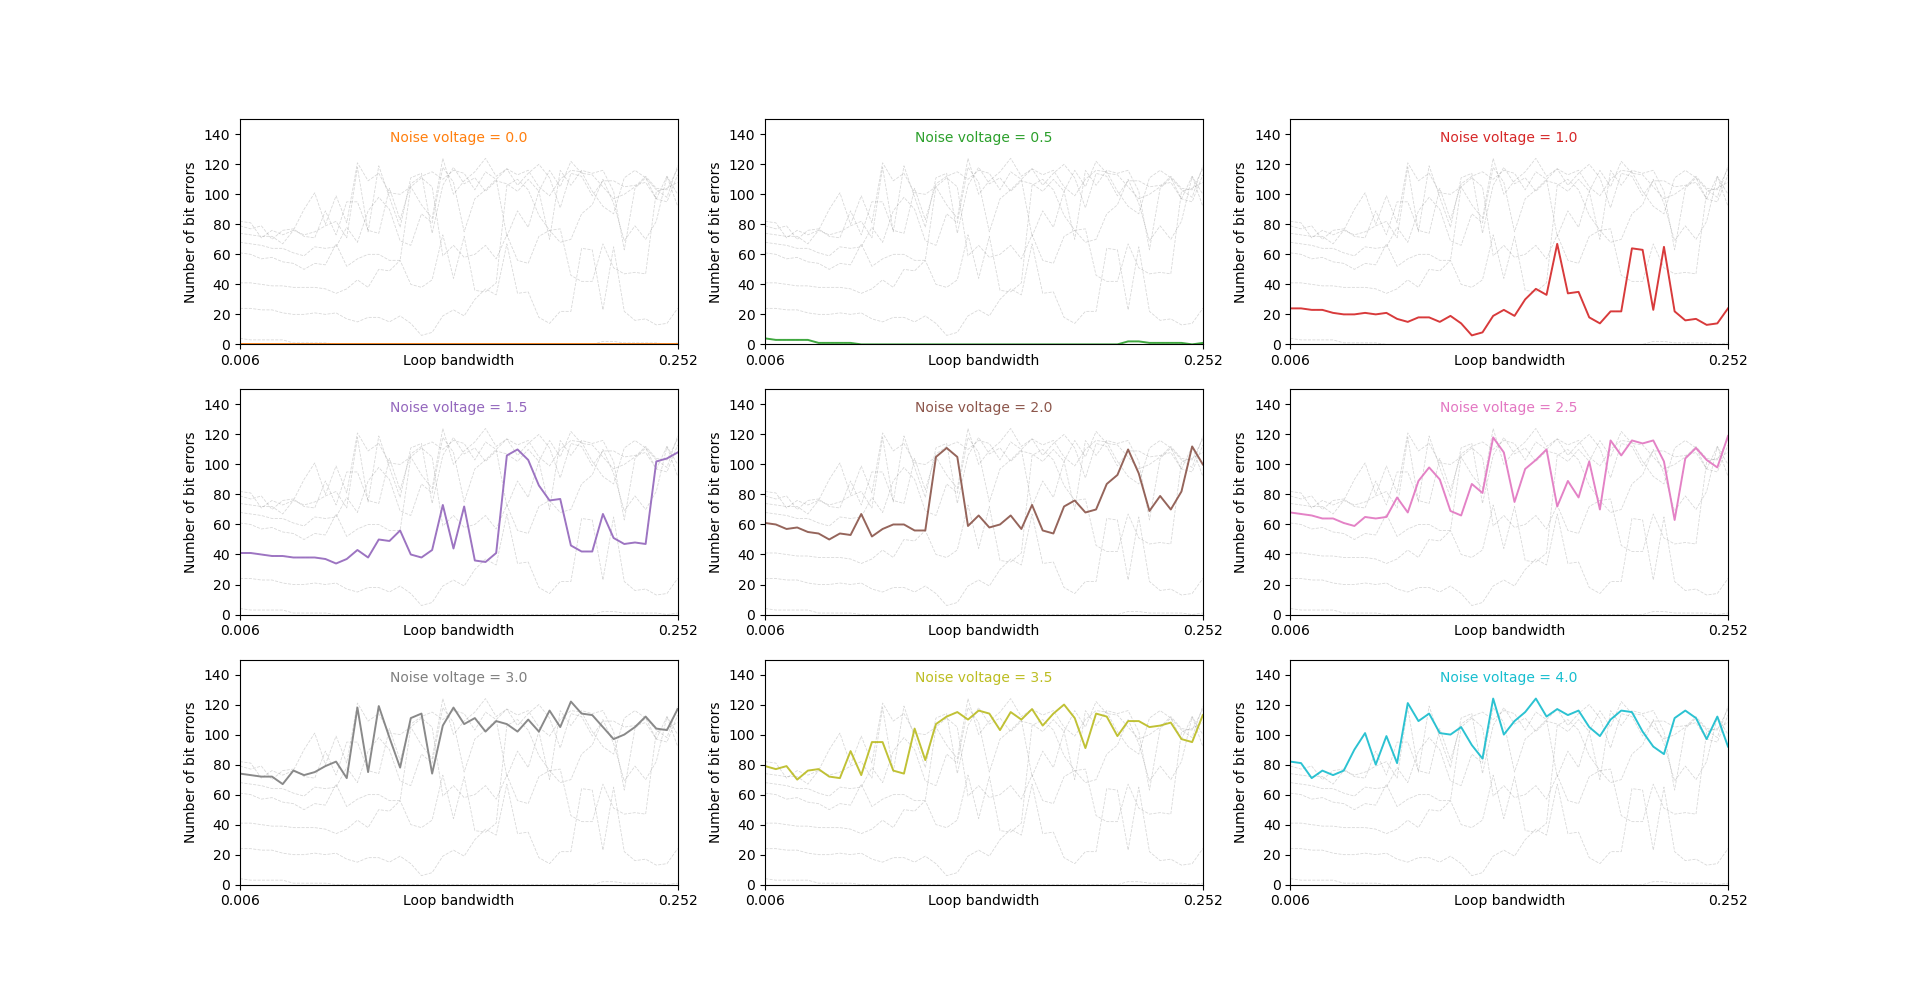
\includegraphics[width=1\linewidth]{img/analise/QPSK_9.png}
    \caption{Evolução do número de erros de bit para cada \textit{noise voltage}, em função da \textit{Loop Bandwidth}.}
    \label{fig:qpsk9}
\end{figure}

\noindent\fcolorbox{black}{white}{%
        \minipage[t]{\dimexpr\linewidth-2\fboxsep-2\fboxrule\relax}
            \textbf{Nota} $\rightarrow$ Os resultados e observações são bastante análogos à versão BPSK, pelo que se seguem as mesmas ilações. Salienta-se somente, para reforçar a ideia, que em média, a taxa de erro de \textit{bit} para cada patamar de ruído impõe precisamente a mesma evolução que no caso exposto anteriormente (vide \hyperref[fig:bpsk9]{Fig. E1} e \hyperref[tab:bpsk]{Tab. E1}). 
        \endminipage}
    %\newpage
%=============================--X--=============================%
\renewcommand{\thefigure}{C\arabic{figure}}
\renewcommand{\thetable}{C\arabic{table}}
\setcounter{figure}{0}
\section{Conclusões}
\label{sec:conclusao}
\begin{figure}[ht] 
    \begin{subfigure}[b]{0.5\linewidth}
        \centering
        \includegraphics[width=0.8\linewidth]{img/conclusao/const-byte85-bpsk.png}
        \caption{BPSK sem \textit{noise voltage}.} 
        \label{fig:a} 
        \vspace{1ex}
    \end{subfigure}%% 
    \begin{subfigure}[b]{0.5\linewidth}
        \centering
        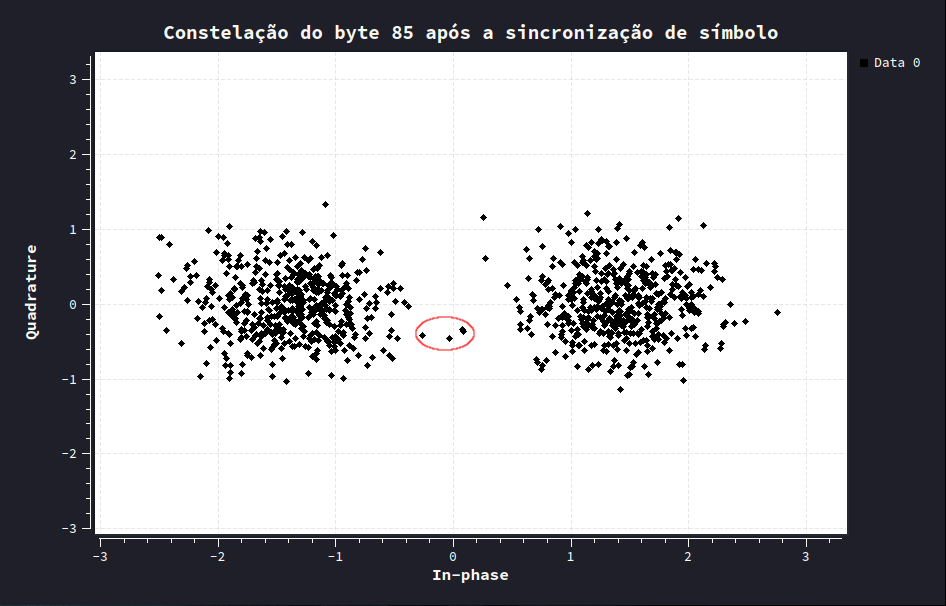
\includegraphics[width=0.8\linewidth]{img/conclusao/const-byte85-bpsk-noisy.png} 
        \caption{BPSK com 0.5 V de \textit{noise voltage}.} 
        \label{fig:b} 
        \vspace{1ex}
    \end{subfigure} 
    \begin{subfigure}[b]{0.5\linewidth}
        \centering
        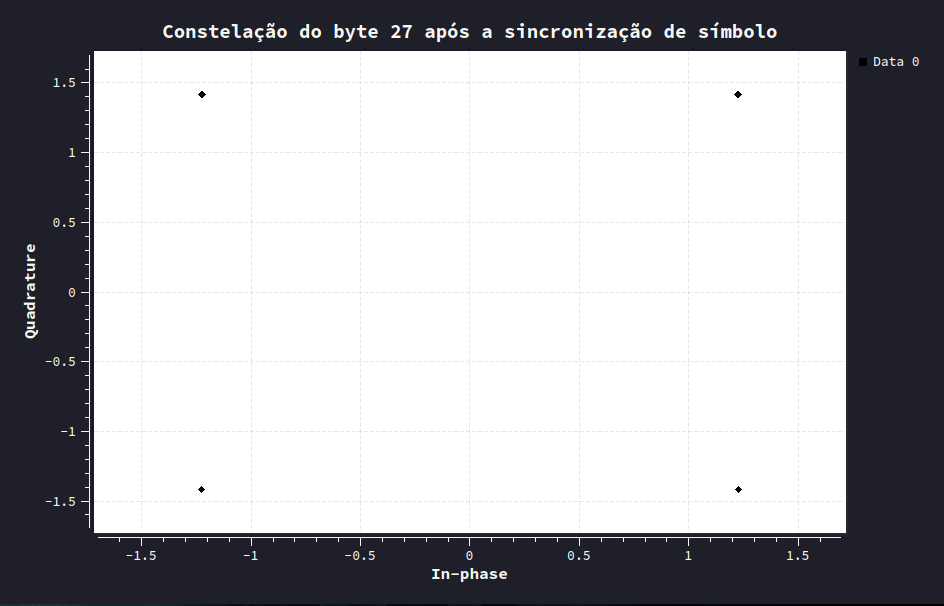
\includegraphics[width=0.8\linewidth]{img/conclusao/const-byte27-qpsk.png}
        \caption{QPSK sem \textit{noise voltage}.} 
        \label{fig:c} 
        %%\vspace{4ex}
    \end{subfigure}%% 
    \begin{subfigure}[b]{0.5\linewidth}
        \centering
        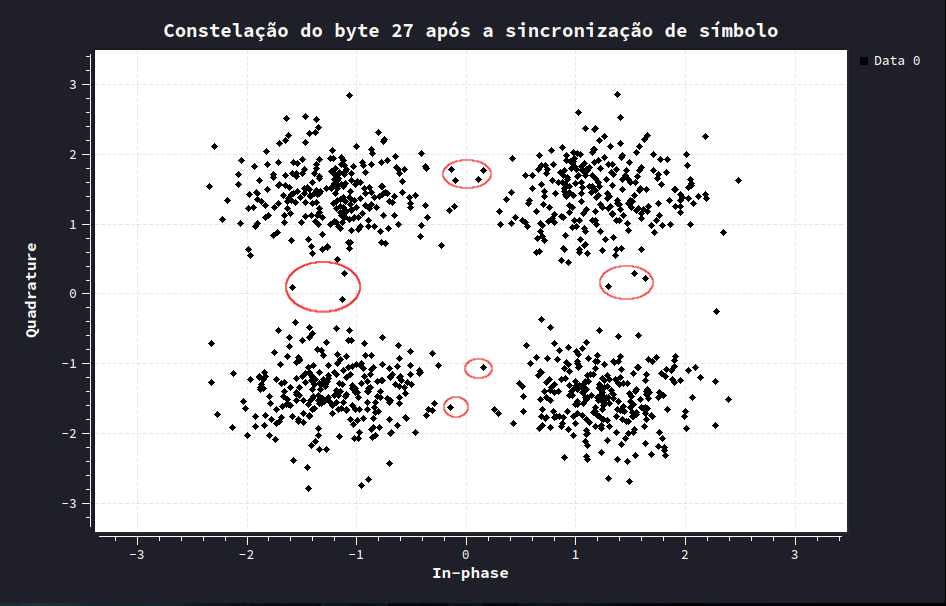
\includegraphics[width=0.8\linewidth]{img/conclusao/const-byte27-qpsk-noisy.png} 
        \caption{QPSK com 0.5 V de \textit{noise voltage}.} 
        \label{fig:d} 
        %%\vspace{4ex}
    \end{subfigure} 
    \caption{Constelações com e sem presença de AWGN.}
    \label{fig:multiplas}
\end{figure}

É conveniente aliar a discussão dos dados obtidos com a visualização dos diagramas de constelação perante a influência de ruído. Na \hyperref[fig:multiplas]{Fig. C1} encontram-se explicitadas a \textcolor{red}{vermelho} amostras situadas numa região de indecisão face à presença de AWGN (ambiguidade na decisão entre \textit{bit} `0' ou `1', vide a \hyperref[subsubsec:stream-to-bit]{secção 3.2}).

Trivialmente se correlacionam os dados adquiridos (ver \hyperref[tab:bpsk]{Tab. E1} e \hyperref[tab:qpsk]{Tab. E2}, e respetivas análises gráfica) com este fenómeno---é aparente que com o aumento do AWGN, há uma tendência (geral) esmagadora, quase obrigatória, para o aumento do número de \textit{bits} nestas zonas litigiosas (graças à dificuldade na deteção do pulso no seio do ruído, como apresentado anteriormente $\xrightarrow[]{}$ redução da relação sinal-ruído).

\begin{figure}[H]
    \centering
    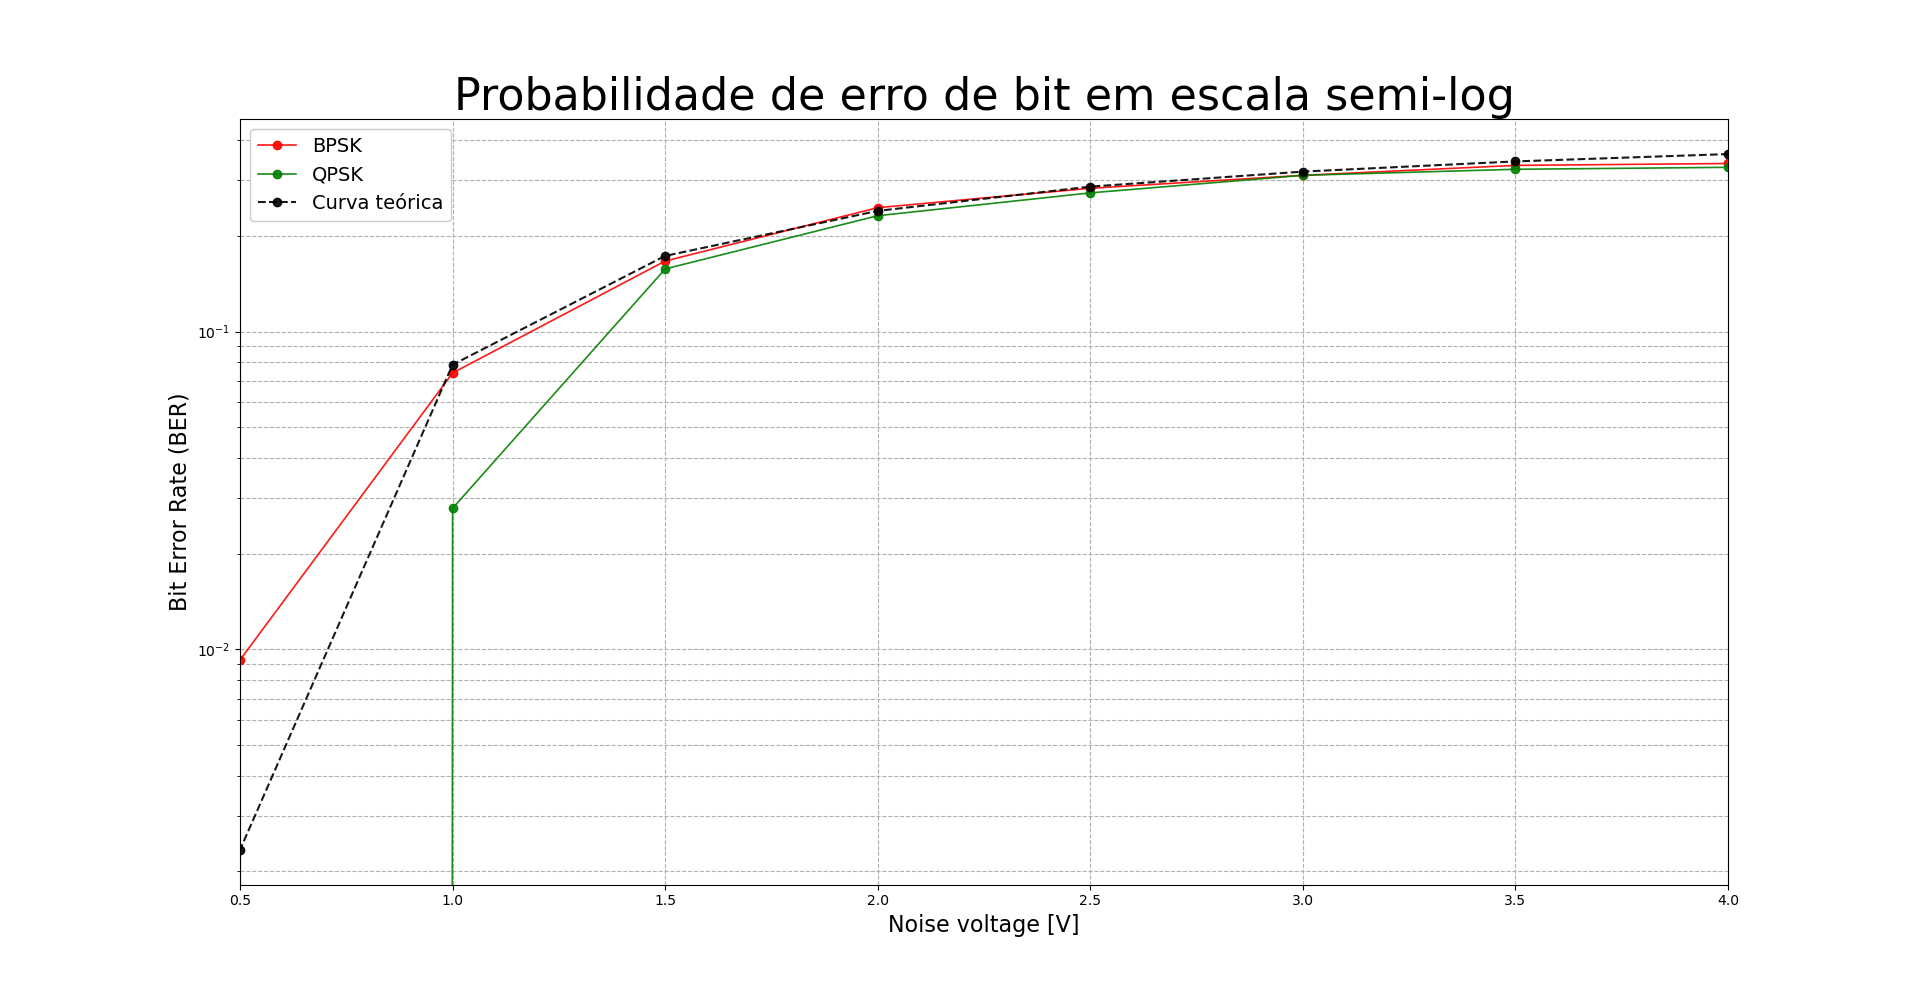
\includegraphics[width=1\linewidth]{img/conclusao/BER_plot.png}
    \caption{Curvas de probabilidade de erro de \textit{bit} (BER) em escala semi-logarítmica: \textcolor{red}{BPSK}, \textcolor{green}{QPSK} e \textcolor{black}{teórica}\protect\footnotemark[12].}
    \label{fig:BERcurves}
\end{figure}

\footnotetext[12]{As curvas \textcolor{red}{BPSK} e \textcolor{green}{QPSK} são computadas mediante a menor taxa de erro de \textit{bit} observada nas tabelas apresentadas para cada patamar de ruído; e a devida curva teórica é obtida com base na expressão supramencionada na \hyperref[subsubsec:prob-erro]{secção 4.1}, aplicada sobre o \textit{range} discreto de \textit{noise voltages} para $\sqrt{E_b} = \sqrt{2}$ (distância à origem visualizada experimentalmente em ambiente \textit{GNU Radio}).}

Não obstante, a sobreposição das curvas apresentadas na \hyperref[fig:BERcurves]{Fig. C2} verifica a similaridade (esperada e bastante proeminente por análise direta das tabelas expostas) entre as probabilidades de erro de \textit{bit} e ratifica o conteúdo teórico---sucintamente condensado na seguinte citação:
\begin{quote}
    "The biggest and primary advantage of QPSK over BPSK is spectral efficiency: for the same BER performance and data rate we can use half the bandwidth! This is also intuitively explained that we are sending two BPSK signals independently in the same bandwidth."\cite{jstraughjstraugh}
\end{quote}
    %% biblio/webgraphy
    \clearpage
    \bibliographystyle{unsrtnat}
    \nocite{*}
    {\footnotesize
    \bibliography{refs}}
    %% attachments
    %\newpage
    %\input{appendix.tex}

\end{document}
